\BourbakiFrontChapter{引言}

数学的多数分支都涉及一类结构，它们不同于本丛书《代数》一书所研究的代数结构（群、环、域等）：即给极限、连续与邻域这些直观概念以数学内容的结构。这些结构正是本书的研究对象。

从历史上看，极限与连续的思想在数学中出现得很早，尤其是在几何学中；随着分析学的发展及其在实验科学中的应用，它们的作用不断增长，因为这些思想与实验测定和近似的思想密切相关。但由于大多数实验测定都是度量，亦即对一个或多个数的测定，因此不足为怪的是，数学中的极限与连续概念起初只出现在实数理论及其衍生物与应用领域（复数、实变量或复变量的实值或复值函数、欧氏几何及有关几何）之中。

近来人们认识到，这些思想的适用范围远远超出了经典分析中的实数与复数（见第一章的历史注记）。通过分析与抽象的努力，它们的本质内容已被提炼出来，其结果是得到一个工具，它在数学的许多分支中的用处已经显而易见。

为了揭示极限、连续与邻域这些思想中的本质内容，我们将从分析邻域概念入手（尽管从历史上看，它比另外两个概念出现得更晚）。如果我们从物理上的近似概念出发，自然可以说：集合 E 的子集 A 是 A 中元素 a 的邻域，如果每当我们用某个“近似”a 的元素代替 a 时，这个新元素也属于 A，当然要假定所涉及的“误差”足够小；或者换句话说，如果 E 中所有“充分接近”a 的点都属于 A。每当能够给“充分小的误差”概念或“一个元素充分接近另一个元素”概念以精确意义时，这个定义就是有意义的。沿这个方向，第一个想法是假定两个元素之间的“距离”可以用一个（正）实数来度量。一旦定义了集合中任意两个元素之间的“距离”，应当如何定义元素 a 的“邻域”便是清楚的了：一个子集将是 a 的邻域，如果它包含所有与 a 的距离小于某个事先给定的严格正数的元素。当然，除非对“距离”附加某些条件或公理（例如，欧氏几何中关于三角形三个顶点之间的距离所成立的不等式，对我们的推广距离仍应成立），否则不能指望由这个定义发展出一个有趣的理论。这样我们就得到了欧氏几何的一个巨大推广。继续使用几何学的语言是方便的：于是，定义了“距离”的集合，其元素称为点，而该集合本身称为空间。我们将在第九章研究此类空间。

到目前为止，我们尚未成功摆脱实数。然而，如此定义的空间具有许许多多性质，陈述这些性质无须涉及产生它们的那个“距离”。例如，包含 a 的一个邻域的每个子集仍是 a 的邻域，a 的两个邻域的交是 a 的邻域。这些性质以及其他性质有大量推论，无须再求助于当初使我们得以定义邻域的“距离”就能推导出来。我们得到的是其中不再提及量或距离的命题。

这样我们终于被引到拓扑空间的一般概念，它不依赖于任何预备的实数理论。我们说集合 E 赋有一个拓扑结构，只要我们以某种方式使 E 的每个元素都对应了 E 的一个子集族，族中的子集称为该元素的邻域——当然要假定这些邻域满足某些条件（拓扑结构的公理）。显然，所加公理的选择在某种程度上是任意的，并且在历史上曾是大量试验的主题（见第一章的历史注记）。最终得到的公理体系对于数学当前的需要而言足够宽泛，又不至于陷入过分而无益的一般性。

赋有拓扑结构的集合称为拓扑空间，其元素称为点。研究拓扑结构的数学分支名称是拓扑学（按词源是“位置的学科”，这并不是一个特别有表现力的名称），如今人们更愿意用这个名称，而不用较早的同义名称 Analysis situs（位置分析）。

为了表述邻域的思想，我们曾从“一个元素充分接近”另一个元素这一模糊概念出发。反过来，拓扑结构现在使我们能够给“某某性质对所有充分接近 a 的点成立”这一说法以精确的意义：按定义，这意味着具有该性质的点所成的集合，在所论的拓扑结构下是 a 的一个邻域。

从邻域概念引出一系列其他概念，对它们的研究属于拓扑学：集合的内部、集合的闭包、集合的边界、开集、闭集等等（见第一章 § 1）。例如，子集 A 是开集，如果只要点 \(a\) 属于 A，所有充分接近 \(a\) 的点就都属于 A；换句话说，如果 A 是它的每个点的邻域。邻域的公理对所有这些概念都有某些推论；例如，两个开集的交是开集（因为我们已假定了 \(a\) 的两个邻域的交是 \(a\) 的邻域）。反过来，我们也可以从这些导出概念之一出发，而不从邻域概念出发；例如，可以假定开集是已知的，并把开集族的性质取作公理（其中一条性质刚才已作为例子陈述过）。然后可以验证，由开集的知识能够重新构造出邻域；邻域的公理现在成为我们取作出发点的新的开集公理的推论。于是，拓扑结构可以用种种基本等价的不同方式来定义。本书将从开集概念出发，因为相应的公理最简单。

一旦定义了拓扑结构，就容易使连续性的观念精确化。直观上，如果只要变元保持在所论点的充分近处，函数的值就变化得要多小有多小，则函数在该点连续。于是，只要函数的变元空间与值空间都是拓扑空间，连续性就有精确的意义。精确的定义在第一章 § 2 中给出。

与连续性一样，极限的观念涉及两个集合，每个都赋有适当的结构，还有一个集合到另一个集合的映射。例如，实数序列 \(a_{n}\) 的极限涉及自然数集合 N、实数集合 R，以及前一集合到后一集合的映射。称实数 a 为该序列的极限，如果无论取 a 的哪个邻域 V，该邻域都包含除 n 的有限多个值以外的所有 \(a_{n}\)；也就是说，如果使 \(a_{n}\) 属于 V 的那些自然数 n 所成的集合是 N 的余集有限的子集。注意，由于谈论的是邻域，R 被假定赋有拓扑结构；至于集合 N，我们让某个特定的子集族扮演特殊角色，即余集有限的那些子集。这是一个一般事实：每当我们谈论极限，考虑的都是映射 \(f\)（从一个集合 \(\mathbf{E}\) 到一个拓扑空间 \(\mathbf{F}\)），并且我们说 \(f\) 以点 \(a\)（\(\mathbf{F}\) 中的点）为极限，如果由这样的元素 \(x\)（属于 \(\mathbf{E}\)）所组成的集合——其像 \(f(x)\) 属于

a 的某个邻域 V {[}此集合正是“逆像” \(\overline{f}^{1}(V)\) {]}——无论邻域 V 如何，都属于 E 的某个事先给定的子集族 F。为使极限概念具有通常归之于它的那些本质性质，族 F 必须满足某些公理，这些公理在第一章 § 6 中陈述。E 的这样的子集族 F 称为 E 上的滤子。滤子的概念与极限的概念不可分离，它也出现在拓扑学的其他场合；例如，拓扑空间中一点的诸邻域构成一个滤子。

对所有这些概念的一般研究是第一章的主要目的。此外，那里还考虑拓扑空间的一些特殊类：满足更多限制性公理的空间，或由其他给定空间通过特定程序得到的空间。

如前所述，集合上的拓扑结构使人能够给“每当 x 充分接近 a 时，x 就具有性质 \(P\{x\}\)”这一说法以精确的意义。但是，除去已定义“距离”的情形，尚不清楚应当给“每一对彼此充分接近的点 x, y 都具有性质 \(P\{x, y\}\)”这一说法以什么意义，因为先验地我们没有比较两个不同点的邻域的手段。而彼此接近的点对这一概念在经典分析中频繁出现（例如，在涉及一致连续性的命题中）。因此，重要的是我们能够在完全一般的情形下给这一概念以精确意义，于是我们被引导去定义比拓扑结构更丰富的结构，即一致结构。它们是第二章的主题。

本卷的其余各章致力于这样的问题：在这些问题中，除拓扑结构或一致结构外，还出现别的结构。例如，赋有适当拓扑（在某种意义上与群结构相容）的群称为拓扑群。拓扑群在第三章中研究，我们将在那里特别看到，每个拓扑群如何可以赋有某些一致结构。

在第四章中，我们把上述原理应用于有理数域。这使我们能够定义实数域；由于其重要性，我们将相当详细地研究它。在随后各章中，我们从实数出发定义某些拓扑空间，它们在拓扑学对经典几何的应用中具有特殊意义：有限维向量空间、球面、射影空间等。我们还考虑与

实数的加法群密切相关的某些拓扑群，我们对它们作公理化的刻画，而这就把我们引导到经典分析中最重要的函数（指数函数、对数函数与三角函数）的定义及初等性质。

在第九章中我们回到一般拓扑空间，但现在有一种新工具，即实数，可供我们支配。我们特别研究拓扑借助于“距离”来定义的空间；这些空间具有一些性质，其中若干不能推广到更一般的空间。在第十章中我们研究拓扑空间到一致空间的映射所成的集合（函数空间）；这些集合在赋以适当的拓扑后具有有趣的性质，这些性质在经典分析中已经起着重要作用。

\chapter{拓扑结构}

\section{开集、邻域、闭集}

\subsection{开集}

定义 1. 集合 X 上的拓扑结构（或更简单地，拓扑）是这样的结构：它由 X 的子集所成之集 D 给出，而 D 具有下列性质（称为拓扑结构的公理）：

\((\mathbf{O}_{\mathbf{I}})\) \(\mathfrak{D}\) 中集合的任何并都是 \(\mathfrak{D}\) 中的集合。

\((\mathbf{O}_{\mathbf{II}})\) \(\mathfrak{D}\) 中集合的任何有限交都是 \(\mathfrak{D}\) 中的集合。

\(\mathfrak{D}\) 中的集合称为由 \(\mathfrak{D}\) 在 \(\mathbf{X}\) 上定义的拓扑结构的开集。

定义 2. 拓扑空间是赋有拓扑结构的集合。

拓扑空间的元素常称为点。当在集合 X 上定义了一个拓扑之后，这个集合称为拓扑空间 X 的底集。

公理 \((\mathrm{O}_{\mathrm{I}})\) 特别蕴含：D 的空子集族之并，即空集，属于 D。公理 \((\mathrm{O}_{\mathrm{II}})\) 蕴含：D 的空子集族之交，即集合 X，属于 D。

拓扑的例子。对任一集合 X，由 X 与 \(\varnothing\) 组成的子集所成之集满足公理 \((\mathrm{O}_{\mathrm{I}})\) 与 \((\mathrm{O}_{\mathrm{II}})\)，因此在 X 上定义了一个拓扑。由 X 的所有子集组成的集合 \(\mathfrak{P}(\mathbf{X})\) 亦然：它定义的拓扑是 X 上的离散拓扑，而赋有该拓扑的集合 X 称为离散空间。

设 \((\mathbf{U}_i)_{i\in I}\) 是 \(\mathbf{A}\)（拓扑空间 \(\mathbf{X}\) 的一个子集）的覆盖；如果所有的 \(\mathbf{U}_i\) 在 \(\mathbf{X}\) 中都是开集，则称该覆盖为开覆盖。

定义 3. 拓扑空间 X 到拓扑空间 X' 上的同胚是 X 的拓扑结构到 X' 的拓扑结构上的同构；也就是说，按照一般定义，它是 X 到 X' 上的一个双射，且把 X 的开子集所成之集变换为 X' 的开子集所成之集。

称 X 与 \(X'\) 同胚，如果存在 X 到 \(X'\) 上的一个同胚。

例。如果 X 与 \(X'\) 是两个离散空间，则 X 到 \(X'\) 上的任何双射都是同胚。

由同胚的定义立即得到下列判别准则：双射 \(f\)（由拓扑空间 \(\mathbf{X}\) 到拓扑空间 \(\mathbf{X}'\) 上）是同胚的充分必要条件是：在 \(f\) 之下，\(\mathbf{X}\) 中每个开集的像是 \(\mathbf{X}'\) 中的开集，并且在 \(f\) 之下，\(\mathbf{X}'\) 中每个开集的逆像是 \(\mathbf{X}\) 中的开集。

\subsection{邻域}

定义 4. 设 X 是拓扑空间，A 是 X 的任一子集。A 的邻域是 X 中包含一个含 A 的开集的任一子集。由单独一点组成的子集 \(\{x\}\) 的邻域也称为点 x 的邻域。

显然，X 的子集 A 的每个邻域也是每个子集 \(B \subset A\) 的邻域；特别地，它是 A 的每个点的邻域。反之，设 A 是集合 B 的每一点的邻域，并设 U 是含于 A 的诸开集之并；则 \(U \subset A\)，且由于 B 的每一点都属于某个含于 A 的开集，我们有 \(B \subset U\)；而由 \((\mathrm{O}_{\mathrm{I}})\)，U 是开集，故 A 是 B 的邻域。特别地：

命题 1. 集合是它的每个点的邻域，当且仅当它是开集。

“邻域”一词的日常含义使得涉及邻域这一数学概念的许多性质表现为直观性质的数学表达；因此选用这个术语的好处是使语言更富有表现力。为此，在某些陈述中还可以使用“充分接近”与“要多接近有多接近”这样的表述。例如，命题 1 可以陈述成如下形式：集合 A 是开集，当且仅当对每个 \(x \in A\)，所有充分接近 x 的点都属于 A。更一般地，如果一个性质在点 x 的某个邻域的所有点处都成立，我们就说该性质在充分接近点 x 的所有点处成立。

用 \(\mathfrak{B}(x)\) 表示 \(x\) 的所有邻域所成之集。诸集合 \(\mathfrak{B}(x)\) 具有下列性质：

\((\mathbf{V}_{\mathbf{I}})\) \(\mathbf{X}\) 中包含一个属于 \(\mathfrak{B}(x)\) 的集合的每个子集，本身属于 \(\mathfrak{B}(x)\)。

\((V_{II})\) \(\mathfrak{B}(x)\) 中集合的每个有限交属于 \(\mathfrak{B}(x)\)。

\((V_{\mathrm{III}})\) 元素 \(x\) 属于 \(\mathfrak{B}(x)\) 的每个集合。

事实上，这三条性质是定义 4 与公理 (O \(_{II}\) ) 的直接推论。

\((V_{IV})\) 如果 V 属于 \(\mathfrak{B}(x)\)，则存在一个属于 \(\mathfrak{B}(x)\) 的集合 W，使得对每个 \(y \in W\)，V 属于 \(\mathfrak{B}(y)\)。

由命题 1，可取 W 为包含 x 且含于 V 的任一开集。

这条性质可以表述为：x 的一个邻域也是充分接近 x 的所有点的邻域。

诸集合 \(\mathfrak{B}(x)\) 的这四条性质是特征性质。确切地说，我们有：

命题 2. 如果对每个元素 \(x\)（属于一个集合 \(\mathbf{X}\)）都对应了一个子集族 \(\mathfrak{B}(x)\)，它由 \(\mathbf{X}\) 的子集组成，且使得性质 \((\mathbf{V}_{\mathbf{I}}), (\mathbf{V}_{\mathbf{II}}), (\mathbf{V}_{\mathbf{III}})\) 与 \((\mathbf{V}_{\mathbf{IV}})\) 成立，则在 \(\mathbf{X}\) 上存在唯一的拓扑结构，使得对每个 \(x \in \mathbf{X}\)，\(\mathfrak{B}(x)\) 是该拓扑中 \(x\) 的邻域全体所成之集。

由命题 1，如果 X 上存在满足这些条件的拓扑，则该拓扑的开集全体必是集合 \(\mathfrak{D}\)——X 的这样的子集 A 所成之集：对每个 \(x \in \mathbf{A}\) 有 \(\mathbf{A} \in \mathfrak{B}(x)\)；由此可得该拓扑（若存在）的唯一性。

集合 \(\mathfrak{D}\) 当然满足公理 \((\mathrm{O_I})\) 与 \((\mathrm{O_{II}})\)：对 \((\mathrm{O_I})\) 而言，这由 \((\mathrm{V_I})\) 立即得出；对 \((\mathrm{O_{II}})\) 而言，则由 \((\mathrm{V_{II}})\) 得出。尚须证明，在由 \(\mathfrak{D}\) 定义的拓扑中，\(\mathfrak{B}(x)\) 是 \(x\) 的邻域全体（对每个 \(x \in \mathbf{X}\)）。由 \((\mathbf{V}_{\mathbf{I}})\)，\(x\) 的每个邻域都属于 \(\mathfrak{B}(x)\)。反之，设 \(\mathbf{V}\) 是属于 \(\mathfrak{B}(x)\) 的一个集合，并设 \(\mathbf{U}\) 是点 \(y \in \mathbf{X}\) 全体所成之集，其中 \(\mathbf{V} \in \mathfrak{B}(y)\)；如果能证明 \(x \in \mathbf{U}\)、\(\mathbf{U} \subset \mathbf{V}\) 与 \(\mathbf{U} \in \mathfrak{D}\)，则证明即告完成。我们有 \(x \in \mathbf{U}\)，因为 \(\mathbf{V} \in \mathfrak{B}(x)\)；又有 \(\mathbf{U} \subset \mathbf{V}\)，因为每个点 \(y \in \mathbf{U}\) 都属于 \(\mathbf{V}\)，这由 \((\mathbf{V}_{\mathbf{III}})\) 与假设 \(\mathbf{V} \in \mathfrak{B}(y)\) 得出。尚须证明 \(\mathbf{U} \in \mathfrak{D}\)，即 \(\mathbf{U} \in \mathfrak{B}(y)\) 对每个 \(y \in \mathbf{U}\) 成立；于是（图 1）若 \(y \in \mathbf{U}\)，则由 \((\mathbf{V}_{\mathbf{IV}})\)，存在一个集合 \(\mathbf{W}\)，使得对每个 \(z \in \mathbf{W}\) 有 \(\mathbf{V} \in \mathfrak{B}(z)\)；由于 \(\mathbf{V} \in \mathfrak{B}(z)\) 意味着 \(z \in \mathbf{U}\)，故得 \(\mathbf{W} \subset \mathbf{U}\)，从而由 \((\mathbf{V}_{\mathbf{I}})\) 得 \(\mathbf{U} \in \mathfrak{B}(y)\)。证毕。

\pandocbounded{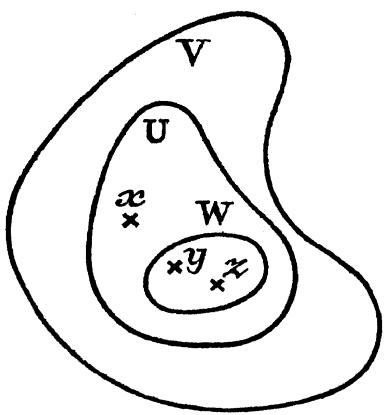
\includegraphics[keepaspectratio]{images/part001_56c83e78.jpg}}\\
图 1.

命题 2 表明，X 上的拓扑可以借助 X 的点的邻域所成之集 \(\mathfrak{B}(x)\) 来定义，只须它们满足公理 \((\mathrm{V}_{\mathrm{I}})\)、\((\mathrm{V}_{\mathrm{II}})\)、\((\mathrm{V}_{\mathrm{III}})\) 与 \((\mathrm{V}_{\mathrm{IV}})\)。

例。我们可以在有理数集合 \(\mathbf{Q}\) 上定义一个拓扑，其开集取为所有有界开区间的并；这些子集所成之集当然满足 \((\mathrm{O}_{\mathbf{I}})\)，而要看出它满足 \((\mathrm{O}_{\mathbf{II}})\)，只须注意：若两个开区间 \(]a, b[\) 与 \(]c, d[\) 的交不空，则它是区间 \(]\alpha, \beta[\)，其中 \(\alpha = \sup (a, c)\) 与 \(\beta = \inf (b, d)\)。对每个 \(x \in \mathbf{Q}\)，把邻域所成之集 \(\mathfrak{B}(x)\)（即 \(x\) 的邻域全体）定义为包含某个含 \(x\) 的开区间的子集全体，就得到同一个拓扑。把该拓扑赋予 \(\mathbf{Q}\) 所得到的拓扑空间称为有理直线（参见第四章，§ 1，第 2 目）。注意，在此空间中每个开区间都是开集。* 我们可以用同样的方式在实数集合 \(\mathbf{R}\) 上定义拓扑；赋有该拓扑的 \(\mathbf{R}\) 称为实直线（参见 § 2，习题 5 及第四章，§ 1，第 3 目）。*

\subsection{基本邻域系；拓扑基}

定义 5. 在拓扑空间 X 中，点 x（相应地，X 的子集 A）的基本邻域系是指 x（相应地，A）的邻域所成的任一集合 S，使得对 x（相应地，A）的每个邻域 V，存在邻域 W ∈ S 满足 W ⊂ V。

如果 \(\mathfrak{S}\) 是子集 \(A\)（\(X\) 的子集）的基本邻域系，则 \(\mathfrak{S}\) 中集合的每个有限交都包含 \(\mathfrak{S}\) 的某个集合。

例。1) 在离散空间（第 1 目）中，单独的集合 \(\{x\}\) 就构成点 \(x\) 的基本邻域系。

\begin{enumerate}
\def\labelenumi{\arabic{enumi})}
\setcounter{enumi}{1}
\tightlist
\item
  在有理直线 Q 上，包含点 x 的所有开区间所成之集是该点的一个基本邻域系。开区间 \(]x - 1/n, x + 1/n[\) 所成之集，以及闭区间 \([x - 1/n, x + 1/n]\) 所成之集亦然，其中 n 取遍所有整数 \textgreater0，或取遍由整数 \textgreater0 组成的任一严格递增无穷序列。* 对实直线有类似的结果。*
\end{enumerate}

定义 6. 拓扑空间 X 的拓扑的拓扑基是指 X 的开子集所成的任一集合 B，使得 X 的每个开子集都是属于 B 的集合之并。

命题 3. 如果 X 是拓扑空间，则 X 的开子集所成的集合 B 是 X 的拓扑的拓扑基的充分必要条件是：对每个 \(x \in X\)，由 \(V \in B\)（其中 \(x \in V\)）所成之集是 x 的基本邻域系。

显然该条件是必要的。反之，若该条件成立，则对任一开集 U 与任一 \(x \in U\)，存在开集 \(V_{x} \in B\) 使得 \(x \in V_{x} \subset U\)。于是诸集合 \(V_{x}\)（对 \(x \in U\)）之并等于 U。证毕。

例。1) 离散拓扑以 X 的由单独一点组成的子集所成之集为一个拓扑基。

\begin{enumerate}
\def\labelenumi{\arabic{enumi})}
\setcounter{enumi}{1}
\tightlist
\item
  有界开区间所成之集依定义是有理直线（第 2 目）的拓扑的一个拓扑基。* 同样，有界开区间所成之集是实直线的拓扑的一个拓扑基。*
\end{enumerate}

\subsection{闭集}

定义 7. 在拓扑空间 X 中，X 的开集的余集称为闭集。

取余集，可知公理 \((\mathbf{O}_{\mathbf{I}})\) 与 \((\mathbf{O}_{\mathbf{II}})\) 取下列形式：

\((\mathbf{O}_{\mathbf{I}}^{\prime})\) 闭集的任何交是闭集。

\((\mathbf{O}_{\mathrm{II}}^{\prime})\) 闭集的任何有限并是闭集。

空集与整个空间 X 都是闭集（从而既开又闭；参见 § 11）。

在有理直线上，每个形如 \([a, \rightarrow[\) 的区间都是闭集，因为它的余集 \(]\leftarrow, a[\) 是开集；同样，每个形如 \(]\leftarrow, a]\) 的区间都是闭集；从而每个有界闭区间 \([a, b]\) 也是闭集，因为它是区间 \([a, \rightarrow[\) 与 \(]\leftarrow, b]\) 之交。

有理整数集 Z 在有理直线中是闭集，因为它的

余集 \(\bigcup_{n\in \mathbf{Z}}]n,n + 1[\) 是开集。

设 \((\mathbf{F}_i)_{i\in I}\) 是 \(\mathbf{A}\)（拓扑空间 \(\mathbf{X}\) 的一个子集）的覆盖；如果每个 \(\mathbf{F}_i\) 在 \(\mathbf{X}\) 中都是闭集，则称该覆盖为闭覆盖。

同胚 \(f\)（由拓扑空间 \(\mathbf{X}\) 到拓扑空间 \(\mathbf{X}'\) 上，第 1 目）可以刻画为 \(\mathbf{X}\) 到 \(\mathbf{X}'\) 上的一个双射，使得在 \(f\) 之下，\(\mathbf{X}\) 的每个闭子集的像是 \(\mathbf{X}'\) 的闭子集，并且在 \(f\) 之下，\(\mathbf{X}'\) 的每个闭子集的逆像是 \(\mathbf{X}\) 的闭子集。

\subsection{局部有限族}

定义 8. 族 \((\mathbf{A}_{i})_{i\in \mathbf{I}}\)（拓扑空间 \(\mathbf{X}\) 的子集所成的族）称为局部有限的，如果对每个 \(x\in \mathbf{X}\)，存在一个邻域 \(\mathbf{V}\)（\(x\) 的邻域），使得 \(\mathbf{V}\cap \mathbf{A}_i = \emptyset\) 对除去有限多个指标 \(i\in \mathbf{I}\) 外成立。子集所成的集合 \(\mathfrak{S}\)（\(\mathbf{X}\) 的子集所成之集）称为局部有限的，如果由 \(\mathfrak{S}\) 到自身的恒等映射所定义的子集族是局部有限的。

显然，如果 \((\mathbf{A}_t)_{t \in \mathbf{I}}\) 是局部有限的子集族，并且 \(\mathbf{B}_t \subset \mathbf{A}_t\) 对每个 \(t \in \mathbf{I}\) 成立，则族 \((\mathbf{B}_t)_{t \in \mathbf{I}}\) 是局部有限的。

拓扑空间的每个有限子集族显然是局部有限的；反之一般不成立。

* 例如，在 R 中，由区间 \(]\leftarrow, 1[\) 与诸区间 \(]n, \rightarrow[\)（对每个整数 \(n\geqslant0\)）所形成的开覆盖是局部有限的；而每个区间 \(]n, \rightarrow[\) 都与该覆盖中的无穷多个集合相交。

命题 4. 拓扑空间 X 的闭子集所成的局部有限族之并在 X 中是闭集。

设 \((\mathbf{F}_i)_{i\in I}\) 是 \(X\) 的闭子集所成的一个局部有限族，并设 \(x\in X\) 不属于 \(\mathbf{F} = \bigcup_{i\in I}\mathbf{F}_i\)；则 \(x\) 有一个邻域 \(V\)，它只与那些 \(\mathbf{F}_i\) 相交，后者的指标属于某个有限子集 \(J\)（\(I\) 的子集）。对每个 \(i\in J\)，设 \(\mathbf{U}_i\) 为 \(\mathbf{F}_i\) 的余集；则 \(\mathbb{CF}\) 包含集合 \(V\cap \bigcap_{i\in J}\mathbf{U}_i\)，后者是 \(x\) 的一个邻域，因为每个 \(\mathbf{U}_i\) 都是开集且包含 \(x\)。于是，由第 2 目的命题 1，\(\mathbb{CF}\) 是开集，从而 \(\mathbf{F}\) 在 \(X\) 中是闭集。

我们注意到，X 的闭子集所成的任意族之并未必是闭集；例如，在有理直线 Q 上，集合 \(]0, 1[\) 是诸闭集

\[
\left[ \frac {1}{n}, 1 - \frac {1}{n} \right] \quad \text { for } n > 2,
\]

之并，但它不是闭集。

\subsection{集合的内部、闭包、边界；稠密集}

定义 9. 在拓扑空间 X 中，点 x 称为 X 的子集 A 的内点，如果 A 是 x 的邻域。A 的内点所成之集称为 A 的内部，记作 \(\mathring{A}\)。

根据定义 9 与定义 4，点 x 是 A 的内点，如果存在包含在 A 中且包含 x 的开集；由此可知 \(\mathring{A}\) 是包含在 A 中的所有开集之并，因而是包含在 A 中的最大开集：换言之，若 B 是包含在 A 中的开集，则 B ⊂ \(\mathring{A}\)。从而，若 A 与 B 是 X 的两个子集且 B ⊂ A，则 \(\mathring{B} \subset \mathring{A}\)；并且 A 是 B 的邻域当且仅当 B ⊂ \(\mathring{A}\)。

注. 非空集合的内部可以是空集；例如，由单独一点（该点不是开集）组成的集合就是这种情形，比如在有理直线上 * （或实直线上） *。

第 2 目的命题 1 可以改述如下：

一个集合是开集当且仅当它与自己的内部相重合。

第 2 目的性质 \((V_{II})\) 蕴含：凡是两个子集 A 与 B 中每一个的内点的点，都是 \(A \cap B\) 的内点；从而

\[
\mathring {\mathbf {A} \cap \mathbf {B}} = \mathring {\mathbf {A}} \cap \mathring {\mathbf {B}}.\tag{1}
\]

凡是集合 A 的余集的内点的点称为 A 的外点，这些点所成之集称为 A 在 X 中的外部；因此，点 \(x \in X\) 是 A 的外点这一事实可由下述性质刻画：x 有一个不与 A 相交的邻域。

定义 10. 拓扑空间 X 的子集 A 的闭包是指由所有这样的点 \(x \in X\) 组成的集合：x 的每个邻域都与 A 相交；闭包记作 \(\overline{A}\)。

这个定义可以改述为：点 x 位于集合 A 的闭包中，如果 A 中存在与 x 要多接近就有多接近的点。

凡不属于 A 的闭包的点都是 A 的外点，反之亦然；于是我们有下列（互为对偶的）公式

\[
\mathbf {C} \overline {{\mathbf {A}}} = \mathring {\mathbf {C} \mathbf {A}}, \quad \mathbf {C} \mathring {\mathbf {A}} = \overline {{\mathbf {C} \mathbf {A}}}.\tag{2}
\]

因此，由对偶性，关于集合内部的每个命题都对应一个关于闭包的命题，反之亦然。特别地，集合 A 的闭包是包含 A 的最小闭集；换言之，若 B 是使 \(A \subset B\) 成立的闭集，则 \(\overline{A} \subset B\)。若 A 与 B 是 X 的两个子集且 \(A \subset B\)，则 \(\overline{A} \subset \overline{B}\)。

一个集合是闭集当且仅当它与自己的闭包相重合。

公式 (1) 的对偶是

\[
\overline {{{\mathbf {A} \cup \mathbf {B}}}} = \overline {{{\mathbf {A}}}} \cup \overline {{{\mathbf {B}}}}.\tag{3}
\]

命题 5. 设 A 是 X 中的开集；则对 X 的每个子集 B，我们有

\[
\mathbf {A} \cap \overline {{\mathbf {B}}} \subset \overline {{\mathbf {A} \cap \mathbf {B}}}.\tag{4}
\]

因为设 \(x \in A \cap \overline{B}\)；则若 V 是 x 的任一邻域，\(V \cap A\) 是 x 的邻域（因 A 是开集）；于是 \(V \cap A \cap B\) 非空，从而 x 位于 \(A \cap B\) 的闭包中。

如果 \(x\) 位于 \(A\) 的闭包中但不属于 \(A\)，则 \(x\) 的每个邻域都包含 \(A\) 中一个异于 \(x\) 的点；但若 \(x \in A\)，则可能发生这样的情形：\(x\) 有一个邻域，它不含 \(A\) 的任何异于 \(x\) 的点。这时我们说 \(x\) 是 \(A\) 的孤立点。特别地，\(x\) 在整个空间 \(X\) 中是孤立点当且仅当 \(\{x\}\) 是开集。

没有孤立点的闭集称为完备集。

定义 11. 在拓扑空间 X 中，点 x 称为集合 A 的边界点，如果 x 既位于 A 的闭包中又位于 CA 的闭包中。A 的边界点所成之集称为 A 的边界。

于是 A 的边界是集合 \(\overline{A} \cap \overline{\complement A}\)，它是闭集。A 的边界点 x 可由下述性质刻画：x 的每个邻域至少包含 A 的一个点和 CA 的一个点；x 可以属于 A 也可以不属于 A。A 的边界与 CA 的边界相同。A 的内部、A 的外部与 A 的边界两两不相交，其并是整个空间 X。

定义 12. 拓扑空间 X 的子集 A 称为在 X 中稠密（若关于 X 不会引起混淆，就简称稠密），如果 \(\overline{A} = X\)，亦即如果 X 的每个非空开集 U 都与 A 相交。

例。* 我们将在第四章 § 1 中看到，有理数集及其余集在实直线上都稠密。*

在离散空间 X 中，X 的唯一稠密子集是 \(X^{*}\) 自身。另一方面，在 X 上以 \(\varnothing\) 与 X 为仅有开集的拓扑中，X 的每个非空子集都稠密。

命题 6. 如果 \(\mathfrak{B}\) 是拓扑空间 \(X\) 的拓扑的一个拓扑基，则存在一个稠密集 \(D\)（在 \(X\) 中），使得 \(\operatorname{Card}(D) \leqslant \operatorname{Card}(\mathfrak{B})\)。

我们可以限于 \(\mathfrak{B}\) 中没有集合是空集的情形（\(\mathfrak{B}\) 的非空集合已经构成 \(\mathbf{X}\) 的拓扑的一个拓扑基）。对每个 \(\mathbf{U} \in \mathfrak{B}\)，设 \(x_{\mathbf{U}}\) 是 \(\mathbf{U}\) 的一个点；由第 3 目的命题 3 可知，集合 \(\mathbf{D}\)（由诸点 \(x_{\mathbf{U}}\) 组成）在 \(\mathbf{X}\) 中稠密，并且我们有 Card \((\mathbf{D}) \leqslant\) Card \((\mathfrak{B})\)（《集合论》，第三章，§ 3，第 2 目，命题 3）。

\section{连续函数}

\subsection{连续函数}

定义 1. 映射 \(f\)（由拓扑空间 \(\mathbf{X}\) 到拓扑空间 \(\mathbf{X}'\) 中的映射）称为在点 \(x_0 \in \mathbf{X}\) 处连续，如果对任一邻域 \(\mathbf{V}'\)（\(f(x_0)\) 在 \(\mathbf{X}'\) 中的邻域），存在一个邻域 \(\mathbf{V}\)（\(x_0\) 在 \(\mathbf{X}\) 中的邻域），使得关系 \(x \in \mathbf{V}\) 蕴含 \(f(x) \in \mathbf{V}'\)。

定义 1 可以改述为下列更直观的形式：说 \(f\) 在点 \(x_0\) 处连续，意思是 \(f(x)\) 可以随意地接近 \(f(x_0)\)，只要 \(x\) 充分接近 \(x_0\)。

关系“对每个 \(x \in V\)，\(f(x) \in V'\)”等价于 \(f(V) \subset V'\)，或者再等价于 \(V \subset \overline{f}^{1}(V')\)；鉴于邻域公理 \((V_{I})\)，我们看到定义 1 等价于下述定义：称 \(f: X \to X'\) 在点 \(x_{0}\) 处连续，如果对每个邻域 \(V'\)（\(f(x_{0})\) 在 \(X'\) 中的邻域），\(\overline{f}^{1}(V')\) 是 \(x_{0}\) 在 X 中的邻域。而且，只需 \(\overline{f}^{1}(V')\) 是 \(x_{0}\) 的邻域（对每个邻域 \(V'\)，它属于 \(f(x_{0})\) 在 \(X'\) 中的某个基本邻域系）就够了（§ 1，第 3 目）。

命题 1. 设 \(f\) 是由拓扑空间 \(\mathbf{X}\) 到拓扑空间 \(\mathbf{X}'\) 中的一个映射。如果 \(f\) 在 \(x\) 处连续，并且 \(x\) 位于子集 \(A\)（\(X\) 的子集）的闭包中，则 \(f(x)\) 位于 \(f(A)\) 的闭包中。

设 \(\mathbf{V}'\) 是 \(f(x)\) 在 \(\mathbf{X}'\) 中的一个邻域。由于 \(f\) 在 \(x\) 处连续，\(\overline{f}^1 (\mathbf{V}')\) 是 \(x\) 在 \(\mathbf{X}\) 中的邻域。于是 \(\overline{f}^1 (\mathbf{V}')\) 与 \(\mathbf{A}\) 相交，由此推出 \(\mathbf{V}'\) 与 \(f(\mathbf{A})\) 相交，从而 \(f(x)\) 位于 \(f(\mathbf{A})\) 的闭包中。

命题 2. 设 X、X'、X'' 是三个拓扑空间；设 f 是由 X 到 X' 中的映射，在 x ∈ X 处连续；设 g 是由 X' 到 X'' 中的映射，在 f(x) 处连续。则复合映射 h = g \(\circ\) f: X → X'' 在 x 处连续。

设 \(V''\) 是 \(h(x) = g(f(x))\) 在 \(X''\) 中的一个邻域。由于 \(g\) 在 \(f(x)\) 处连续，可知 \(\overline{g}^1(V'')\) 是 \(f(x)\) 在 \(X'\) 中的邻域。但 \(f\) 在 \(x\) 处连续，故 \(\overline{f}^1(\overline{g}^1(V'')) = \overline{h}^1(V'')\) 是 \(x\) 在 \(X\) 中的邻域，从而 \(h\) 在 \(x\) 处连续。

定义 2. 由拓扑空间 X 到拓扑空间 X' 中的映射称为在 X 上连续（或简称连续），如果它在 X 的每一点都连续。

例。1) 拓扑空间 X 到自身的恒等映射是连续的。

\begin{enumerate}
\def\labelenumi{\arabic{enumi})}
\setcounter{enumi}{1}
\item
  拓扑空间到拓扑空间中的常映射是连续的。
\item
  由离散空间到拓扑空间中的每个映射都是连续的。
\end{enumerate}

定理 1. 设 \(f\) 是由拓扑空间 \(X\) 到拓扑空间 \(X'\) 中的一个映射。则下列命题等价：

\begin{enumerate}
\def\labelenumi{\alph{enumi})}
\item
  \(f\) 在 \(\mathbf{X}\) 中连续。
\item
  对 X 的每个子集 A，\(f(\overline{\mathrm{A}}) \subset \overline{f(\mathrm{A})}\)。
\item
  在 \(f\) 之下，\(\mathbf{X}'\) 的每个闭子集的逆像是 \(\mathbf{X}\) 的闭子集。
\item
  在 \(f\) 之下，\(\mathbf{X}'\) 的每个开子集的逆像是 \(\mathbf{X}\) 的开子集。
\end{enumerate}

我们已经看到 a) 蕴含 b)（命题 1）。为证 b) 蕴含 c)，设 \(\mathbf{F}'\) 是 \(\mathbf{X}'\) 的闭子集，并设 \(\mathbf{F} = \overline{f}^{1}(\mathbf{F}')\)；则由假设 \(f(\overline{\mathbf{F}}) \subset \overline{f(\mathbf{F})} \subset \overline{\mathbf{F}}' = \mathbf{F}'\)，故 \(\overline{\mathbf{F}} \subset \overline{f}^{1}(\mathbf{F}') = \mathbf{F} \subset \overline{\mathbf{F}}\)，于是 \(\mathbf{F} = \overline{\mathbf{F}}\)，即 \(\mathbf{F}\) 是闭集。鉴于关系式 \(\complement \overline{f}^{1}(A') = \overline{f}^{1}(\complement A')\)（对每个子集 \(A'\)（\(X'\) 的子集）成立），c) 蕴含 d)。最后，设 d) 成立。设 \(x\) 是 \(X\) 的任一点，并设 \(V'\) 是 \(f(x)\) 在 \(X'\) 中的任一邻域；则存在开集 \(A'\)（\(X'\) 中的），使得

\[
f (x) \in \mathrm{A} ^ {\prime} \subset \mathrm{V} ^ {\prime}
\]

从而 \(x \in \overline{f}^1(\mathbf{A}') \subset \overline{f}^1(\mathbf{V}')\)。由假设，\(\overline{f}^1(\mathbf{A}')\) 在 \(\mathbf{X}\) 中是开集，于是 \(\overline{f}^1(\mathbf{V}')\) 是 \(x\) 在 \(\mathbf{X}\) 中的邻域。这样 d) 蕴含 a)。

注。1) 设 \(\mathfrak{B}\) 是 \(\mathbf{X}'\) 的拓扑的一个拓扑基（§ 1，第 3 目）；则为使 \(f: \mathbf{X} \to \mathbf{X}'\) 连续，必要且充分的是：\(\overline{f}^1(\mathbf{U}')\) 在 \(\mathbf{X}\) 中是开集（对每个 \(\mathbf{U}' \in \mathfrak{B}\)）。

例。设 \(a\) 是任一有理数。映射 \(x \to a + x\)（由有理直线 \(\mathbf{Q}\) 到自身的映射）在 \(\mathbf{Q}\) 上连续，因为开区间 \(]b, c[\) 在该映射下的逆像是开区间

\[
] b - a, c - a [.
\]

同样，映射 \(x \to ax\) 在 \(\mathbf{Q}\) 上连续；若 \(a = 0\) 这是显然的，因为此时 \(ax = 0\) 对所有 \(x\) 成立；若 \(a \neq 0\)，则开区间 \(]b, c[\) 在该映射下的逆像是以 \(b / a\) 与 \(c / a\) 为端点的开区间。

\pandocbounded{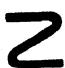
\includegraphics[keepaspectratio]{images/part001_4077020d.jpg}}

\begin{enumerate}
\def\labelenumi{\arabic{enumi})}
\setcounter{enumi}{1}
\tightlist
\item
  在连续映射 \(f: \mathbf{X} \to \mathbf{X}'\) 下，X 的开（相应地，闭）集的直接像在 \(\mathbf{X}'\) 中未必是开（相应地，闭）集（参见 § 5）。
\end{enumerate}

例。* 映射 \(f: x \to 1 / (1 + x^2)\)（由 \(\mathbf{R}\) 到自身的映射）是连续的，但 \(f(\mathbf{R})\) 是半开区间 {[}0, 1{]}，它在 \(\mathbf{R}\) 中既不是开集也不是闭集。*

定理 2. 1) 如果 \(f: \mathbf{X} \to \mathbf{X}'\) 与 \(g: \mathbf{X}' \to \mathbf{X}''\) 是两个连续映射，则 \(g \circ f: \mathbf{X} \to \mathbf{X}''\) 连续。

\begin{enumerate}
\def\labelenumi{\arabic{enumi})}
\setcounter{enumi}{1}
\tightlist
\item
  为使双射 \(f\)（由拓扑空间 \(X\) 到拓扑空间 \(X'\) 上的双射）是同胚，必要且充分的是 \(f\) 与 \(f\) 的逆都连续（或者说，\(f\) 是双连续的）。
\end{enumerate}

第一个断言是命题 2 的直接推论；第二个断言由定理 1 的 d) 与同胚的定义（§ 1，第 1 目）得出。

\pandocbounded{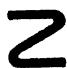
\includegraphics[keepaspectratio]{images/part001_720050f1.jpg}}

注。1) 可能存在由拓扑空间 X 到拓扑空间 X' 上的连续双射而不是双连续的：例如，取 X' 为有理直线 Q，取 X 为赋予离散拓扑的集合 Q；则恒等映射 X → X' 连续但不是同胚。

\begin{enumerate}
\def\labelenumi{\arabic{enumi})}
\setcounter{enumi}{1}
\item
  为验证连续双射 \(f: \mathbf{X} \to \mathbf{X}'\) 是同胚，只需证明：对每个 \(x \in \mathbf{X}\) 与每个邻域 \(V\)（\(x\) 的邻域），\(f(V)\) 是 \(f(x)\) 在 \(\mathbf{X}'\) 中的邻域。
\item
  设 X 是拓扑空间，对每个 \(x \in X\)，设 \(\mathfrak{B}(x)\) 是 x 的所有邻域所成之集。设 \(x_{0}\) 是 X 的一点；对每个 \(x \in X\)，按如下方式定义 X 的子集所成之集 \(\mathfrak{B}_{0}(x)\)：\(\mathfrak{B}_{0}(x_{0}) = \mathfrak{B}(x_{0})\)，而若 \(x \neq x_{0}\)，则 \(\mathfrak{B}_{0}(x)\) 取为 X 的包含 x 的所有子集所成之集。立即可以验证（§ 1，第 2 目，命题 2），诸集 \(\mathfrak{B}_{0}(x)\) 是 X 上某个拓扑的诸点的邻域集；用 \(X_{0}\) 表示这样得到的拓扑空间，用 \(j : X_{0} \to X\) 表示恒等映射，它连续但一般不是双连续的。X 到拓扑空间 \(X'\) 中的映射 f 在点 \(x_{0}\) 处连续当且仅当复合映射 \(X_{0} \stackrel{j}{\to} X \stackrel{f}{\to} X'\) 在 \(X_{0}\) 上连续；这由定义立即得出。
\end{enumerate}

\subsection{拓扑的比较}

第 1 目的定理 2 表明，我们可以把连续映射取作拓扑结构的态射（《集合论》，第四章，§ 2，第 1 目）；从现在起，我们假定已作出了这样的态射选取。按照一般定义（《集合论》，第四章，§ 2，第 2 目），这使我们可以对给定集合 X 上的诸拓扑所成之集定义一个序：

定义 3. 给定同一集合 X 上的两个拓扑 \(\mathfrak{C}_1\)、\(\mathfrak{C}_2\)，我们说 \(\mathfrak{C}_1\) 比 \(\mathfrak{C}_2\) 细（而 \(\mathfrak{C}_2\) 比 \(\mathfrak{C}_1\) 粗），如果记 \(X_i\) 为赋以拓扑 \(\mathfrak{C}_i\)（\(i = 1, 2\)）的集合 X，恒等映射 \(X_1 \to X_2\) 连续。若此外还有 \(\mathfrak{C}_1 \neq \mathfrak{C}_2\)，则说 \(\mathfrak{C}_1\) 比 \(\mathfrak{C}_2\) 严格地细（而 \(\mathfrak{C}_2\) 比 \(\mathfrak{C}_1\) 严格地粗）。

两个拓扑，若其中一个比另一个细，则称它们是可比较的。

映射连续性的判别法（第 1 目，定义 1 与定理 1）给出下列命题：

命题 3. 给定两个拓扑 \(\mathfrak{G}_1\)、\(\mathfrak{G}_2\)（集合 \(X\) 上的拓扑），下列命题等价：

\begin{enumerate}
\def\labelenumi{\alph{enumi})}
\item
  \(\mathfrak{C}_1\) 比 \(\mathfrak{C}_2\) 细。
\item
  对每个 \(x \in \mathbf{X}\)，\(x\) 关于 \(\mathfrak{C}_2\) 的每个邻域都是 \(x\) 关于 \(\mathfrak{C}_1\) 的邻域。
\item
  对 X 的每个子集 A，A 在拓扑 \(C_{1}\) 中的闭包包含在 A 在拓扑 \(C_{2}\) 中的闭包之中。
\item
  在 \(\mathfrak{C}_{2}\) 中为闭集的 X 的每个子集在 \(\mathfrak{C}_{1}\) 中也是闭集。
\item
  在 \(\mathfrak{C}_{2}\) 中为开集的 X 的每个子集在 \(\mathfrak{C}_{1}\) 中也是开集。
\end{enumerate}

例。* 在由实数的序列 \(x = (x_n)\) 组成的 Hilbert 空间 H 中，这些序列满足

\[
\| x \| ^ {2} = \sum_ {n = 0} ^ {\infty} x _ {n} ^ {2} <   + \infty ,
\]

点 \(x_0\) 在 H 上的强拓扑中的邻域是包含开球 \(\|x - x_0\| < a\)（以 \(x_0\) 为中心的开球）的集合；\(x_0\) 在 H 上的弱拓扑中的邻域是包含由形如 \(\sup_{1 \leqslant i \leqslant n} |(x - x_0|a_i)| \leqslant 1\) 的关系所定义之集的集合，其中诸 \(a_i\) 是 H 的点，并且

\[
(x | y) = \sum_ {n = 0} ^ {\infty} x _ {n} y _ {n}
\]

（若 \(x = (x_n)\) 且 \(y = (y_n)\)）。现在若 \(\beta = \sup_{1 \leqslant i \leqslant n} \|a_i\|\)，则关系 \(\|x - x_0\| \leqslant 1/\beta\) 蕴含 \(|(x - x_0|a_i)| \leqslant \|x - x_0\| \cdot \|a_i\| \leqslant 1\)（对 \(1 \leqslant i \leqslant n\)）；因此 H 上的强拓扑比弱拓扑细。另一方面，对 H 的点的任意有限族 \((a_i)_{1 \leqslant i \leqslant n}\)，存在 H 中的点 \(x\)，使 \((x - x_0|a_i) = 0\)（对 \(1 \leqslant i \leqslant n\)）且使 \(\|x - x_0\|\) 任意大；这表明强拓扑比弱拓扑严格地细。*

注。1) 在集合 X 上所有拓扑组成的有序集中，仅以 \(\varnothing\) 与 X 为开集的拓扑是最粗的，而离散拓扑是最细的。

\begin{enumerate}
\def\labelenumi{\arabic{enumi})}
\setcounter{enumi}{1}
\item
  拓扑越细，开集、闭集与邻域就越多；拓扑越细，集合的闭包（相应地，内部）就越小（相应地，越大）；拓扑越细，稠密集就越少。
\item
  如果 \(f: \mathbf{X} \to \mathbf{X}'\) 是连续映射，那么当把 \(\mathbf{X}\) 的拓扑换成较细的拓扑、把 \(\mathbf{X}'\) 的拓扑换成较粗的拓扑时，它仍然连续（第 1 目，定理 2）。换言之，\(\mathbf{X}\) 的拓扑越细且 \(\mathbf{X}'\) 的拓扑越粗，由 \(\mathbf{X}\) 到 \(\mathbf{X}'\) 中的连续映射就越多。
\end{enumerate}

\subsection{初始拓扑}

命题 4. 设 X 是一个集合，设 \((\mathbf{Y}_i)_{i \in I}\) 是拓扑空间的一个族，并且对每个 \(i \in I\)，设 \(f_i\) 是由 X 到 \(\mathbf{Y}_i\) 中的一个映射。设 \(\mathfrak{S}\) 是 X 的形如 \(\overline{f}_i^1 (\mathbf{U}_i)\)（\(i \in I\)，\(\mathbf{U}_i\) 在 \(\mathbf{Y}_i\) 中开）的子集所成之集，并设 \(\mathfrak{B}\) 是 \(\mathfrak{S}\) 的集合的有限交所成之集。则 \(\mathfrak{B}\) 是 X 上某个拓扑 \(\mathfrak{C}\) 的拓扑基，该拓扑是 X 关于族 \((f_i)\) 的初始拓扑结构（《集合论》，第四章，§ 2，第 3 目），特别地，它是使诸映射 \(f_i\) 连续的 X 上最粗的拓扑。更精确地说，若 \(g\) 是由拓扑空间 Z 到 X 中的映射，则 \(g\) 在某点 \(z \in Z\) 处连续（X 赋以拓扑 \(\mathfrak{C}\)）当且仅当每个函数 \(f_i \circ g\) 都在 \(z\) 处连续。

设 \(\mathfrak{D}\) 是属于 \(\mathfrak{B}\) 的集合的所有并所成之集；显然 \(\mathfrak{D}\) 满足公理 \((\mathrm{O}_{\mathrm{I}})\)，因为取并的运算是可结合的；而 \(\mathfrak{D}\) 满足公理 \((\mathrm{O}_{\mathrm{II}})\)，这是由于 \(\mathfrak{B}\) 的定义以及有限交对任意并的分配律 {[}Set Theory, R § 4, formula (37){]}。于是集合 \(\mathfrak{D}\) 是 X 关于某个拓扑 \(\mathfrak{G}\) 的开子集所成之集，\(\mathfrak{B}\) 是该拓扑的一个拓扑基。我们将证明命题的最后一个断言，由初始结构的一般性质（《集合论》，第四章，§ 2，第 3 目，判别准则 CST 9），它蕴含其余断言。首先，\(\mathfrak{S}\) 的定义表明诸 \(f_{i}\) 在 X 上连续（第 1 目，定理 1）；因此，若 \(g\) 在 \(z\) 处连续，则诸映射 \(f_{i} \circ g\) 亦然（第 1 目，命题 2）。反之，设所有映射 \(f_{i} \circ g\) 都在 \(z\) 处连续，并设 V 是 \(g(z)\) 在 X 中的一个邻域；按定义，存在 I 的一个有限子集 J，并且对每个 \(i \in J\)，存在开子集 \(\mathrm{U}_{i}\)（\(\mathrm{Y}_{i}\) 的开子集），使得 V 包含集合 \(\bigcap_{i \in J} f_{i}^{1}(\mathrm{U}_{i})\) 且 \(g(z)\) 属于这个集合。由此推出

\[
\overline {{g}} ^ {1} (\mathrm{V}) \supset \bigcap_ {i \in J} \overline {{g}} ^ {1} (\overline {{f}} _ {i} ^ {1} (\mathrm{U} _ {i})),
\]

而假设蕴含诸集合 \(\overline{g}^{1}(\overline{f}_{i}^{1}(\mathbf{U}_{i}))\) 中的每一个都是 \(z\) 在 \(\mathbf{Z}\) 中的邻域；于是 \(\overline{g}^{1}(\mathbf{V})\) 也是 \(z\) 在 \(\mathbf{Z}\) 中的邻域。证毕。

设 \(\mathfrak{B}_i\) 是 \(\mathbf{Y}_i(t\in I)\) 的拓扑的一个拓扑基；用 \(\mathfrak{S}'\) 表示 \(X\) 的形如 \(\overline{f}_i^1 (U_i)\) 的子集所成之集（对 \(t\in I\) 且 \(U_{t}\in \mathfrak{B}_{t}\)（对每个 \(t\in I\)））；若 \(\mathfrak{B}'\) 是 \(\mathfrak{S}'\) 的集合的有限交所成之集，则显然 \(\mathfrak{B}'\) 是拓扑 \(\mathfrak{C}\) 的一个拓扑基。

初始结构的一般性质（《集合论》，第四章，§ 2，第 3 目，判别准则 CST 10）特别地蕴含下列传递性质（其直接证明是十分容易的）：

命题 5. 设 X 是一个集合，\((Z_{t})_{t\in I}\) 是拓扑空间的一个族，\((J_{\lambda})_{\lambda\in L}\) 是 I 的一个分拆，而 \((Y_{\lambda})_{\lambda\in L}\) 是以 L 为指标的一族集合。又对每个 \(\lambda\in L\)，设 \(h_{\lambda}\) 是由 X 到 \(Y_{\lambda}\) 中的一个映射；对每个 \(\lambda\in L\) 与每个 \(t\in J_{\lambda}\)，设 \(g_{t\lambda}\) 是由 \(Y_{\lambda}\) 到 \(Z_{t}\) 中的一个映射，并令 \(f_{t}=g_{t\lambda}\circ h_{\lambda}\)。如果每个 \(Y_{\lambda}\) 都赋以使诸映射 \(g_{t\lambda}(t\in J_{\lambda})\) 连续的最粗拓扑，那么使诸 \(f_{t}\) 连续的 X 上最粗的拓扑与使诸 \(h_{\lambda}\) 连续的最粗拓扑相同。

例。1) 拓扑的逆像。设 X 是一个集合，Y 是拓扑空间，f 是由 X 到 Y 中的映射；使 f 连续的 X 上最粗的拓扑 C 称为 Y 的拓扑在 f 下的逆像。由命题 4 以及并与交的逆像公式 {[}Set Theory, R, § 4, formulae (34) and (46){]} 可知，拓扑 C 中的开（相应地，闭）集是 Y 的开（相应地，闭）集在 f 下的逆像；从而，对每个 \(x \in X\)，诸集合 \(\overline{f}^{1}(W)\)（其中 W 取遍 \(f(x)\) 在 Y 中的某个基本邻域系）构成 x 在拓扑 C 中的基本邻域系。在 § 3 中我们将以诱导拓扑之名研究 X 是 Y 的子集且 f 是典范单射 \(X \to Y\) 这一特殊情形；这时赋以诱导拓扑的 X 称为 Y 的子空间。

为使映射 \(f\)（由拓扑空间 \(\mathbf{X}\) 到拓扑空间 \(\mathbf{X}'\) 中的映射）连续，必要且充分的是 \(\mathbf{X}\) 的拓扑比 \(f\) 之下 \(\mathbf{X}'\) 的拓扑的逆像细。

\begin{enumerate}
\def\labelenumi{\arabic{enumi})}
\setcounter{enumi}{1}
\tightlist
\item
  拓扑集的上确界。拓扑的每个族 \((\mathcal{C}_t)_{i\in I}\)（集合 \(X\) 上的拓扑的族）都有一个上确界 \(\mathcal{C}\)（在 \(X\) 上所有拓扑的有序集中），即存在 \(X\) 上的一个拓扑，它在 \(X\) 上比每个 \(\mathcal{C}_t\) 都细的所有拓扑中是最粗的。为看出这一点，可以应用命题 4，取 \(Y_t\) 为集合 \(X\)（赋以拓扑 \(\mathcal{C}_t\)），取 \(f_t\) 为恒等映射 \(X\to Y_t\)；\(\mathcal{C}\) 是使所有映射 \(f_t\) 连续的最粗拓扑。
\end{enumerate}

设 \(\mathfrak{S}\) 是集合 X 的子集的任意集合；在 X 上的诸拓扑 \(\mathfrak{C}\)（使 \(\mathfrak{S}\) 的集合皆为开集者）中，有一个拓扑 \(\mathfrak{C}_0\) 比其他所有拓扑都粗，称为由 \(\mathfrak{S}\) 生成的拓扑。对每个集合 \(U \in \mathfrak{S}\)，设 \(\mathfrak{C}_U\) 为以 \(\varnothing\)、U 与 X 为开集的拓扑{[}显然 X 的这个子集集合满足 \((O_I)\) 与 \((O_{II})]\)；则 \(\mathfrak{C}_0\) 恰是诸拓扑 \(\mathfrak{C}_U\) 的上确界。由命题 4，若 \(\mathfrak{B}\) 是属于 \(\mathfrak{S}\) 的集合的有限交所成之集，则 \(\mathfrak{B}\) 是拓扑 \(\mathfrak{C}_0\) 的一个拓扑基。我们说 \(\mathfrak{S}\) 是 \(\mathfrak{C}_0\) 的一个子基。

\begin{enumerate}
\def\labelenumi{\arabic{enumi})}
\setcounter{enumi}{2}
\tightlist
\item
  积拓扑。设 \((\mathbf{X}_t)_{i \in I}\) 是拓扑空间的一个族。积集合 \(\mathbf{X} = \prod_{i \in I} \mathbf{X}_i\) 上使诸
\end{enumerate}

投影 \(pr_{i}: X \rightarrow X_{i}\) 为连续映射的最粗拓扑称为诸 \(X_{i}\) 的拓扑之积；我们将在 § 4 中更详细地研究它。

\subsection{终拓扑}

命题 6. 设 X 是一个集合，设 \((\mathbf{Y}_t)_{t \in I}\) 是拓扑空间的一个族，并且对每个 \(t \in I\)，设 \(f_t\) 是由 \(\mathbf{Y}_t\) 到 X 中的映射。设 \(\mathfrak{D}\) 是 X 的这样的子集 U 所成之集：\(\overline{f}_t^1(\mathbf{U})\) 在 \(\mathbf{Y}_t\) 中是开集（对每个 \(t \in I\)）；则 \(\mathfrak{D}\) 是 X 上某个拓扑 \(\mathfrak{C}\) 的开子集所成之集，该拓扑是 X 关于族 \((f_t)\) 的终结构（《集合论》，第四章，§ 2，第 5 目），特别地，\(\mathfrak{C}\) 是使诸映射 \(f_t\) 连续的 X 上最细的拓扑。换言之，若 g 是由 X 到拓扑空间 Z 中的映射，则 g 连续（X 赋以拓扑 \(\mathfrak{C}\)）当且仅当每个映射 \(g \circ f_t\) 连续。

立即可以验证 \(\mathfrak{D}\) 满足公理 \((\mathrm{O_I})\) 与 \((\mathrm{O_{II}})\)。{[}Set Theory, R, § 4, formulae (34) and (46){]}。我们将证明命题的最后一个断言，由终结构的一般性质（《集合论》，第四章，§ 2，第 5 目，判别准则 CST 18），它蕴含其余断言。显然诸 \(f_{i}\) 在拓扑 \(\mathfrak{C}\) 中连续，这由 \(\mathfrak{D}\) 的定义得出（第 1 目，定理 1）；因此若 \(g\) 连续，则每个映射 \(g \circ f_{i}\) 连续（第 1 目，定理 2）。反之，设每个 \(g \circ f_{i}\) 都连续，并设 V 是 Z 中的开集；由假设，\(\overline{f}_{i}^{1}(\overline{g}^{1}(V))\) 在 \(Y_{i}\) 中是开集（对每个 \(i \in I\)）；于是 \(\overline{g}^{1}(V) \in \mathfrak{D}\)，证明完成。

推论. 在命题 6 的假设下，X 的子集 F 在拓扑 \(\mathfrak{C}\) 中是闭集当且仅当 \(\overline{f}_{\iota}^{1}(\mathbf{F})\) 在 \(Y_{\iota}\) 中是闭集（对每个 \(\iota \in I\)）。这由拓扑 \(\mathfrak{C}\) 中开集的定义取余集得出。

终结构的一般性质（《集合论》，第四章，§ 2，第 5 目，判别准则 CST 19）蕴含下列传递性质（其直接证明同样是容易的）：

命题 7. 设 X 是一个集合，\((Z_{\iota})_{\iota \in I}\) 是拓扑空间的一个族，\((J_{\lambda})_{\lambda \in L}\) 是 I 的一个分拆，而 \((Y_{\lambda})_{\lambda \in L}\) 是以 L 为指标的一族集合。又对每个 \(\lambda \in L\)，设 \(h_{\lambda}\) 是由 \(Y_{\lambda}\) 到 X 中的一个映射；对每个 \(\lambda \in L\) 与每个 \(\iota \in J_{\lambda}\)，设 \(g_{\lambda \iota}\) 是由 \(Z_{\iota}\) 到 \(Y_{\lambda}\) 中的一个映射，并令 \(f_{\iota} = h_{\lambda} \circ g_{\lambda \iota}\)。如果每个 \(Y_{\lambda}\) 都赋以使诸映射 \(g_{\lambda \iota} (\iota \in J_{\lambda})\) 连续的最细拓扑，那么使诸 \(f_{\iota}\) 连续的 X 上最细的拓扑与使诸 \(h_{\lambda}\) 连续的最细拓扑相同。

\paragraph*{例}

\begin{enumerate}
\def\labelenumi{\arabic{enumi})}
\item
  商拓扑。设 X 是拓扑空间，R 是 X 上的一个等价关系，Y = X/R 是 X 关于关系 R 的商集，\(\varphi: X \to Y\) 是典范映射。使 \(\varphi\) 连续的 Y 上最细的拓扑称为 X 的拓扑被关系 R 的商；我们将在 § 3 中更详细地研究它。
\item
  拓扑集的下确界。拓扑的每个族 \((\mathfrak{C}_t)_{i \in I}\)（集合 \(X\) 上的拓扑的族）都有一个下确界 \(\mathfrak{C}\)（在 \(X\) 上所有拓扑的集合中），即 \(\mathfrak{C}\) 是 \(X\) 上比每个 \(\mathfrak{C}_t\) 都粗的所有拓扑中最细的一个。为看出这一点，可以应用命题 6，取 \(Y_t\) 为集合 \(X\)（赋以拓扑 \(\mathfrak{C}_t\)），取 \(f_t\) 为恒等映射 \(Y_t \to X\)。若 \(\mathfrak{D}_t\) 是 \(X\) 的在拓扑 \(\mathfrak{C}_t\) 中为开集的子集所成之集，则集合 \(\bigcap_{i \in I} \mathfrak{D}_t\) 是 \(X\) 的在 \(\mathfrak{C}\) 中为开集的子集所成之集。
\end{enumerate}

\(\mathfrak{G}\) 也称为诸拓扑 \(\mathfrak{G}_{t}\) 的交。

\begin{enumerate}
\def\labelenumi{\arabic{enumi})}
\setcounter{enumi}{2}
\tightlist
\item
  拓扑空间的和。设 \((\mathbf{X}_t)_{i \in I}\) 是拓扑空间的一个族，\(\mathbf{X}\) 是诸 \(\mathbf{X}_t\) 的和所成的集合（《集合论》，第二章，§ 4，第 8 目，定义 8）；对每个 \(i \in I\)，设 \(j_t\) 是由 \(\mathbf{X}_t\) 到 \(\mathbf{X}\) 中的典范（单射）映射。最细拓扑 \(\mathfrak{G}\)（\(\mathbf{X}\) 上的、使诸映射 \(j_t\) 连续者）称为诸 \(\mathbf{X}_t\) 的拓扑之和，而 \(\mathbf{X}\) 赋以这个拓扑后称为诸拓扑空间 \(\mathbf{X}_t\) 的和。让我们把每个 \(\mathbf{X}_t\) 与 \(\mathbf{X}\) 的一个子集借助 \(j_t\) 等同起来；则集合 \(\mathbf{A} \subset \mathbf{X}\) 在拓扑 \(\mathfrak{G}\) 中是开（相应地，闭）集当且仅当诸集合 \(\mathbf{A} \cap \mathbf{X}_t\) 中的每一个在 \(\mathbf{X}_t\) 中都是开（相应地，闭）集。特别地，诸 \(\mathbf{X}_t\) 中的每一个都既开又闭。
\end{enumerate}

下列命题推广了例 3 的情形：

命题 8. 设 X 是一个集合，\((\mathbf{X}_{\lambda})_{\lambda \in \mathbf{L}}\) 是 X 的子集的一个族。假设每个 \(X_{\lambda}\) 都赋有一个拓扑 \(C_{\lambda}\)，使得对每对指标 \((\lambda, \mu)\)：

\begin{enumerate}
\def\labelenumi{\arabic{enumi})}
\item
  \(\mathbf{X}_{\lambda} \cap \mathbf{X}_{\mu}\) 在拓扑 \(\mathfrak{C}_{\lambda}, \mathfrak{C}_{\mu}\) 的每一个中都是开（相应地，闭）集。
\item
  在 \(\mathbf{X}_{\lambda} \cap \mathbf{X}_{\mu}\) 上由 \(\mathfrak{C}_{\lambda}\) 与 \(\mathfrak{C}_{\mu}\) 诱导的拓扑相重合。设 \(\mathfrak{C}\) 是 \(\mathbf{X}\) 上使诸单射 \(j_{\lambda}: \mathbf{X}_{\lambda} \to \mathbf{X}\) 连续的最细拓扑。则对每个 \(\lambda \in \mathbf{L}\)，\(\mathbf{X}_{\lambda}\) 在 \(\mathbf{X}\) 中在拓扑 \(\mathfrak{C}\) 下是开（相应地，闭）集，并且 \(\mathfrak{C}\) 在 \(\mathbf{X}_{\lambda}\) 上诱导的拓扑与 \(\mathfrak{C}_{\lambda}\) 相重合。
\end{enumerate}

鉴于命题 6 及其推论，只需证明：对每个 \(\lambda\) 与每个子集 \(A_{\lambda}\)（\(X_{\lambda}\) 的子集），下列命题等价：

\begin{enumerate}
\def\labelenumi{(\roman{enumi})}
\item
  \(\mathbf{A}_{\lambda}\) 在拓扑 \(\mathfrak{C}_{\lambda}\) 中是开（相应地，闭）集。
\item
  对每个 \(\mu \in L\)，\(A_{\lambda} \cap X_{\mu}\) 在拓扑 \(\mathfrak{G}_{\mu}\) 中是开（相应地，闭）集。
\end{enumerate}

显然，取 \(\mu = \lambda\) 即可看出 (ii) 蕴含 (i)。反之，若 (i) 成立，则 \(A_{\lambda} \cap X_{\mu}\) 在 \(X_{\lambda} \cap X_{\mu}\) 中相对于拓扑 \(\mathcal{C}_{\lambda\mu}\) 是开（相应地，闭）集；该拓扑在 \(X_{\lambda} \cap X_{\mu}\) 上由 \(\mathcal{C}_{\lambda}\) 诱导；但 \(\mathcal{C}_{\lambda\mu}\) 也是在 \(X_{\lambda} \cap X_{\mu}\) 上由 \(\mathcal{C}_{\mu}\) 诱导的拓扑；因此 \(A_{\lambda} \cap X_{\mu}\) 也是 \(X_{\lambda} \cap X_{\mu}\) 与一个子集 \(B_{\mu}\) 的交，其中该子集是 \(X_{\mu}\) 的子集且在拓扑 \(\mathcal{C}_{\mu}\) 中是开（相应地，闭）集；由于 \(X_{\lambda} \cap X_{\mu}\) 在 \(\mathcal{C}_{\mu}\) 中是开（相应地，闭）集，\(A_{\lambda} \cap X_{\mu}\) 也如此。证明完毕。

注意，若诸 \(\mathbf{X}_{\lambda}\) 的并不同于 \(\mathbf{X}\)，则 \(\mathcal{G}\) 在 \(\mathbf{X} - \left(\bigcup_{\lambda \in \mathbf{L}} \mathbf{X}_{\lambda}\right)\) 上诱导的拓扑是离散的。这是因为，若 \(x \in \mathbf{X}\) 不属于诸 \(\mathbf{X}_{\lambda}\) 中的任何一个，则 \(\{x\} \cap \mathbf{X}_{\lambda} = \emptyset\) 在每个拓扑 \(\mathcal{G}_{\lambda}\) 中都是开集，因而 \(\{x\}\) 在拓扑 \(\mathcal{G}\) 中是开集。

\subsection{拓扑空间的粘合}

设 \((\mathbf{X}_{\lambda})_{\lambda \in L}\) 是一个集合族，且设 \(\mathbf{X}\) 为作为诸 \(\mathbf{X}_{\lambda}\) 之和的那个集合（《集合论》第二章，§ 4，第 8 目，定义 8）；我们将把每个 \(\mathbf{X}_{\lambda}\) 与 \(\mathbf{X}\) 的一个子集（借助典范单射 \(j_{\lambda}: \mathbf{X}_{\lambda} \to \mathbf{X}\)）等同起来。

设 R 是 X 上的一个等价关系，使得 R 的每个等价类在每个 \(X_{\lambda}\) 中至多有一个元素；对每对指标 \((\lambda, \mu)\)，设 \(A_{\lambda\mu}\) 为 \(X_{\lambda}\) 的由这样的元素 x（存在属于 x 的等价类的元素 \(y \in X_{\mu}\)）组成的子集。显然，对每个 \(x \in A_{\lambda\mu}\)，对应着唯一的与 x 模 R 同余的 \(y \in A_{\mu\lambda}\)；如此定义的映射 \(h_{\mu\lambda}: A_{\lambda\mu} \to A_{\mu\lambda}\) 满足下列条件：

\begin{enumerate}
\def\labelenumi{(\roman{enumi})}
\item
  对每个 \(\lambda \in L\)，\(h_{\lambda \lambda}\) 是 \(\mathbf{A}_{\lambda \lambda} = \mathbf{X}_{\lambda}\) 上的恒等映射。
\item
  对指标的三元组 \((\lambda, \mu, \nu)\)（\(\mathbf{L}\) 中的三元组）以及每个 \(x \in \mathbf{A}_{\lambda \mu} \cap \mathbf{A}_{\lambda \nu}\)，我们有 \(h_{\mu \lambda}(x) \in \mathbf{A}_{\mu \nu}\)，并且
\end{enumerate}

\[
h _ {\nu \lambda} (x) = h _ {\nu \mu} (h _ {\mu \lambda} (x)).\tag{1}
\]

反之，假设对每对指标 \((\lambda, \mu)\) 给定了一个子集 \(A_{\lambda \mu}\)（\(X_{\lambda}\) 的子集）和一个满足上述条件 (i) 与 (ii) 的映射 \(h_{\mu \lambda}: A_{\lambda \mu} \to A_{\mu \lambda}\)。首先，把 (ii) 应用于三元组 \((\lambda, \mu, \lambda)\) 与 \((\mu, \lambda, \mu)\) 可知，\(h_{\lambda \mu} \circ h_{\mu \lambda}\)（相应地，\(h_{\mu \lambda} \circ h_{\lambda \mu}\)）是 \(h_{\lambda \lambda}\)（相应地，\(h_{\mu \mu}\)）在 \(A_{\lambda \mu}\)（相应地，\(A_{\mu \lambda}\)）上的限制；于是由 (i) 推出，\(h_{\lambda \mu}\) 与 \(h_{\mu \lambda}\) 是互为逆映射的双射。现在设 \(R\{x, y\}\) 是关系"存在 \(\lambda, \mu\) 使得 \(x \in A_{\lambda \mu}, y \in A_{\mu \lambda}\) 且 \(y = h_{\mu \lambda}(x)\)"。由 (i) 以及前文可知 \(R\) 是自反的且对称的；另一方面，若 \(x \in A_{\lambda \mu}\)，

\[
y = h _ {\mu \lambda} (x) \in A _ {\mu \lambda} \cap A _ {\mu \nu} \quad \text { and } \quad z = h _ {\nu \mu} (y),
\]

则也有 \(x = h_{\lambda \mu}(y)\)，从而由 (ii) 得 \(x \in A_{\lambda \mu} \cap A_{\lambda \nu}\)；于是关系式 (1) 表明 \(R\) 是传递的，因此 \(R\) 是 \(X\) 上的一个等价关系。由 (i) 以及 \(R\) 的定义还可得出：模 \(R\) 的每个等价类在诸集合 \(X_{\lambda}\) 的每一个中至多有一个元素，并且 \(A_{\lambda \mu}\) 是由所有这样的 \(x \in X_{\lambda}\)（存在元素 \(y \in X_{\mu}\) 与 \(x \mod R\) 同余）组成的集合。我们说，商集 \(X / R\) 是把诸 \(X_{\lambda}\) 沿 \(A_{\lambda \mu}\) 借助诸双射 \(h_{\mu \lambda}\) 粘合在一起而得到的。若 \(\varphi: X \to X / R\) 是典范映射，则 \(\varphi\) 在每个 \(X_{\lambda}\) 上的限制是由 \(X_{\lambda}\) 到 \(\varphi(X_{\lambda})\) 上的一个双射。

现在假设每个 \(X_{\lambda}\) 都是拓扑空间，并设 \(G_{\lambda}\) 为它的拓扑。设 G 为集合 X/R 上使诸映射 \(\varphi \circ j_{\lambda}\) 连续的最细拓扑；G 是 X 上作为诸拓扑 \(G_{\lambda}\) 之和的那个拓扑经 R 得到的商。我们说，拓扑空间 X/R（带拓扑 G）是把诸拓扑空间 \(X_{\lambda}\) 沿 \(A_{\lambda\mu}\) 借助诸双射 \(h_{\mu\lambda}\) 粘合在一起而得到的。于是，X/R 的开（相应地，闭）子集是 X 的子集 B（关于 R 饱和，且 \(B \cap X_{\lambda}\) 在 \(X_{\lambda}\) 中是开（相应地，闭）集（对每个 \(\lambda \in L\)））的典范像。

由于 \(\varphi\) 在每个 \(\mathbf{X}_{\lambda}\) 上的限制是到子集 \(\mathbf{X}_{\lambda}^{\prime} = \varphi (\mathbf{X}_{\lambda})\)（\(\mathbf{X} / \mathbf{R}\) 的子集）上的一个双射，我们可以借助这个双射把拓扑 \(\mathfrak{C}_{\lambda}\) 搬运到 \(\mathbf{X}_{\lambda}^{\prime}\) 上，使 \(\mathbf{X}_{\lambda}^{\prime}\) 带有拓扑 \(\mathfrak{C}_{\lambda}^{\prime}\)；而拓扑 \(\mathfrak{C}\)（\(\mathbf{X} / \mathbf{R}\) 上的拓扑）是使典范单射 \(\mathbf{X}_{\lambda}^{\prime} \to \mathbf{X} / \mathbf{R}\) 连续的最细拓扑。一般地，\(\mathfrak{C}\) 在 \(\mathbf{X}_{\lambda}^{\prime}\) 上诱导的拓扑比 \(\mathfrak{C}_{\lambda}^{\prime}\) 粗，但与后者不恒等；即使诸 \(h_{\mu \lambda}\) 是同胚（§ 3，习题 15）亦然。然而，由第 4 目命题 8 可得，沿用前面的记号：

命题 9. 假设诸 \(h_{\mu \lambda}\) 都是同胚，且每个 \(\mathbf{A}_{\lambda \mu}\) 在 \(\mathbf{X}_{\lambda}\) 中是开（相应地，闭）集；则每个 \(\varphi(\mathbf{X}_{\lambda})\) 在 \(\mathbf{X}/\mathbf{R}\) 中是开（相应地，闭）集，且 \(\varphi\) 在 \(\mathbf{X}_{\lambda}\) 上的限制是由 \(\mathbf{X}_{\lambda}\) 到子空间 \(\varphi(\mathbf{X}_{\lambda})\)（\(\mathbf{X}/\mathbf{R}\) 的子空间）上的一个同胚。

\section{子空间；商空间}

\subsection{拓扑空间的子空间}

设 A 是拓扑空间 X 的一个子集。我们已把 X 的拓扑在 A 上诱导的拓扑定义为该拓扑在典范单射 \(A \rightarrow X\) 下的逆像（§ 2，第 3 目，例 1）。一个等价的定义如下：

定义 1. 设 A 是拓扑空间 X 的一个子集。X 的拓扑在 A 上诱导的拓扑是这样的拓扑，其中的开集是 X 的开集与 A 的交。赋以这个拓扑的集合 A 称为 X 的一个子空间。

例。有理直线的拓扑在有理整数集 Z 上诱导的拓扑是离散拓扑，因为 Z 与开区间 \(]n - 1/2, n + 1/2[\) 的交是集合 \(\{n\}\)。

由 § 2 第 3 目命题 5（或直接由定义 1）可以看出，若 B ⊂ A ⊂ X，则 X 的子空间 B 与 X 的子空间 A 的子空间 B 恒同（诱导拓扑的传递性）。若 S 是 X 的拓扑的一个子基（相应地，拓扑基）（§ 2，第 3 目，例 3），则它在 A 上的迹 \(\mathfrak{S}_{\mathrm{A}}\) 是在 A 上诱导的拓扑的一个子基（相应地，拓扑基）。

在所有涉及 A 的元素或子集的问题中，务必仔细区分它们作为 X 的点（相应地，子集）的性质与它们作为子空间 A 的点（相应地，子集）的性质。我们将用"在 A 中"、"关于 A"或"相对于 A"这些说法来指后一类的性质（必要时把它们与"在 X 中"、"关于 X"、"相对于 X"诸说法相对照）。

子空间 A 的开集不必在 X 中是开集；为使 A 中的每个开集都在 X 中是开集，必须且只需 A 在 X 中是开集。该条件是必要的，因为 A 在 A 中是开集；而由 \((\mathrm{O}_{\mathrm{II}})\) 与定义 1，它又是充分的。

A 中的闭集是 X 中的闭集与 A 的交（§ 2，第 3 目，例 1）；与上面一样，我们看出，A 中的每个闭集在 X 中是闭集当且仅当 A 在 X 中是闭集。

点 \(x \in A\) 相对于 A 的诸邻域是 x 相对于 X 的诸邻域与 A 的交。x 相对于 A 的每个邻域都是 x 相对于 X 的邻域，当且仅当 A 是 x 在 X 中的一个邻域。

命题 1. 若 A 与 B 是拓扑空间 X 的两个子集，且 \(B \subset A\)，则 B 在子空间 A 中的闭包是 B 在 X 中的闭包 \(\overline{B}\) 与 A 的交。

若 \(x \in A\)，则 x 在 A 中的每个邻域都有 \(V \cap A\) 的形式，其中 V 是 x 在 X 中的一个邻域。由于 \(V \cap B = (V \cap A) \cap B\)，由此得出，x 属于 B 相对于 A 的闭包当且仅当 x 属于 B 相对于 X 的闭包。

推论. A 的子集 B 在 A 中稠密，当且仅当在 X 中 \(\overline{B} = \overline{A}\)（亦即当且仅当 \(A \subset \overline{B}\)）。

由此推出，若 A、B、C 是 X 的三个子集，满足 \(A \supset B \supset C\)，且 B 在 A 中稠密，C 在 B 中稠密，则 C 在 A 中稠密（稠密性的传递性），因为在 X 中有 \(\overline{A} = \overline{B} = \overline{C}\)。

命题 2. 设 A 是拓扑空间 X 的一个稠密子集；则对每个 \(x \in \mathbf{A}\) 以及 \(x\) 相对于 A 的每个邻域 V，V 在 X 中的闭包 \(\overline{\mathbf{V}}\) 是 \(x\) 在 X 中的一个邻域。

因为 V 包含 U ∩ A，其中 U 是 X 的包含 x 的开子集，故 \(\overline{V}\) 包含 U ∩ \(\overline{A} = U\)（§ 1，第 6 目，命题 5）。

命题 3. 设 \((\mathbf{A}_i)_{i\in I}\) 是拓扑空间 \(\mathbf{X}\) 的子集的一个族，使得下列性质之一成立：

\begin{enumerate}
\def\labelenumi{\alph{enumi})}
\item
  诸 \(A_{i}\) 的内部覆盖 X。
\item
  \((\mathbf{A}_{\iota})_{\iota \in \mathbf{I}}\) 是 \(\mathbf{X}\) 的一个局部有限闭覆盖（\(\S 1\)，第 5 目）。
\end{enumerate}

在这些条件下，X 的子集 B 在 X 中是开（相应地，闭）集，当且仅当诸集合 \(B \cap A_{t}\) 中的每一个在 \(A_{t}\) 中都是开（相应地，闭）集。

显然，若 B 在 X 中是开（相应地，闭）集，则 \(B \cap A_{t}\) 在 \(A_{t}\) 中是开（相应地，闭）集。反之，先设条件 a) 满足；由于 \((\mathbb{C}\mathbf{B}) \cap \mathbf{A}_{t} = \mathbf{A}_{t} - (\mathbf{B} \cap \mathbf{A}_{t})\)，由对偶性，只需考虑每个 \(B \cap A_{t}\) 相对于 \(A_{t}\) 为开集的情形。在这一情形，\(B \cap \mathring{A}_{t}\) 在 \(\mathring{A}_{t}\) 中是开集（对每个 \(t \in I\)），从而在 X 中是开集；又由假设有 \(B = \bigcup_{i} (B \cap \mathring{A}_{t})\)，故 B 在 X 中是开集。

现在设 b) 满足；再由对偶性，只需考虑每个 \(B \cap A_{t}\) 在 \(A_{t}\) 中是闭集、从而在 X 中是闭集的情形。由于族 \((B \cap A_{t})\) 局部有限且 \(\mathbf{B} = \bigcup_{t} (B \cap A_{t})\)，由 §1 第 5 目命题 4 可知，B 在 X 中是闭集。

注. 设 \((\mathbf{U}_i)_{i\in I}\) 是拓扑空间 \(\mathbf{X}\) 的一个开覆盖，且对每个 \(i\in I\)，设 \(\mathfrak{B}_i\) 是子空间 \(\mathbf{U}_i\)（\(\mathbf{X}\) 的子空间）的拓扑的一个基；则显然 \(\mathfrak{B} = \bigcup_{i\in I}\mathfrak{B}_i\) 是 \(\mathbf{X}\) 的拓扑的一个基。

\subsection{相对于子空间的连续性}

设 X 与 Y 是两个拓扑空间，f 是 X 到 Y 中的一个映射，B 是 Y 的包含 \(f(\mathbf{X})\) 的一个子集。诱导拓扑作为初始拓扑的定义（§ 2，第 3 目，命题 4）表明，f 在 \(x \in X\) 处连续，当且仅当 X 到 Y 的子空间 B 中的、与 f 有同一图象的那个映射在 x 处连续。

现在设 A 是 X 的一个子集；若 f 在 \(x \in A\) 处连续（相应地，在 X 上连续），则它的限制 \(f|A\) 是子空间 A 到 Y 中的一个映射，由 §2 第 1 目命题 2，它在 x 处连续（相应地，在 A 上连续）。我们有时会说，映射 \(f: X \to Y\) 在 \(x \in A\) 处相对于 A 连续（相应地，相对于 A 连续），如果它的限制 \(f|A\) 在 x 处连续（相应地，在 A 上连续）。

应当注意，\(f|A\) 可以连续而 \(f\) 不在 \(X\) 的任何点连续；这种现象的一个例子由特征函数 \(\varphi_A\)（子集 \(A\)（\(X\) 的子集）的特征函数，该子集使 \(A\) 与它的余集都在 \(X\) 中稠密（§ 2，习题 11））给出，其中 \(\varphi_A\) 被看作 \(X\) 到离散空间 \(\{0, 1\}\) 中的一个映射。\(\varphi_A\) 不在 \(X\) 的任何点连续，但它在 \(A\) 上的限制是常数，因而是连续的。

若 A 是点 \(x \in A\) 在 X 中的一个邻域，且 \(f: X \to Y\) 使 \(f|A\) 在 x 处连续，则 f 在 x 处连续；因为 x 在 A 中的每个邻域都是 x 在 X 中的邻域（连续性的局部特征）。

命题 4. 设 \((\mathbf{A}_t)_{i\in I}\) 是拓扑空间 \(\mathbf{X}\) 的子集的一个族，其诸内部覆盖 \(\mathbf{X}\)，或者它是 \(\mathbf{X}\) 的一个局部有限闭覆盖。设 \(f\) 是 \(\mathbf{X}\) 到拓扑空间 \(\mathbf{X}'\) 中的一个映射。若 \(f\) 在每个子空间 \(\mathbf{A}_t\) 上的限制都连续，则 \(f\) 连续。

因为，若 \(\mathbf{F}'\) 是 \(\mathbf{X}'\) 的一个闭子集且 \(\mathbf{F} = \overline{f}^{1} (\mathbf{F}')\)，则 \(\mathbf{F} \cap \mathbf{A}_i\) 在 \(\mathbf{A}_i\) 中是闭集（对每个 \(i \in I\)）（\(\S 2\)，第 1 目，定理 1），因而由第 1 目命题 3，\(\mathbf{F}\) 在 \(\mathbf{X}\) 中是闭集；于是结论由 \(\S 2\) 第 1 目定理 1 得出。

\subsection{局部闭子空间}

定义 2. 称拓扑空间 X 的子集 L 在点 \(x \in L\) 处是局部闭的，如果存在 x 在 X 中的一个邻域 V，使得 \(L \cap V\) 是子空间 V 的一个闭子集。若 L 在每个 \(x \in L\) 处都是局部闭的，则称 L 在 X 中是局部闭的。

注. 设 F 是 X 的一个子集，使得对 X 的每个点 x 存在 x 的一个邻域 V 满足 \(V \cap F\) 在子空间 V 中是闭集；则由第 1 目命题 3，F 在 X 中是闭集。另一方面，下面的命题 5 表明，一般存在在 X 中不闭的局部闭集。

命题 5. 对拓扑空间 X 的子集 L 而言，下列诸性质等价：

\begin{enumerate}
\def\labelenumi{\alph{enumi})}
\item
  L 在 X 中是局部闭的。
\item
  L 是 X 的一个开子集与一个闭子集的交。
\item
  L 在它在 X 中的闭包 \(\overline{L}\) 中是开集。
\end{enumerate}

若 L 局部闭，则对每个 \(x \in L\)，存在 x 在 X 中的一个开邻域 \(V_{x}\)，使得 \(L \cap V_{x}\) 在 \(V_{x}\) 中是闭集；\(U = \bigcup_{x \in L} V_{x}\) 在 X 中是开集，且第 1 目命题 3 表明 L 在 U 中是闭集；因此 a) 蕴含 b)。若 \(L = U \cap F\)，其中 U 是开集而 F 在 X 中是闭集，则有 \(\overline{L} \subset F\)；于是 \(L \subset U \cap \overline{L} \subset U \cap F = L\)，这表明 \(L = U \cap \overline{L}\) 在 \(\overline{L}\) 中是开集，故 b) 蕴含 c)。最后，若 \(L = U \cap \overline{L}\)，其中 U 在 X 中是开集，则 \(\overline{L}\) 在 U 中是闭集，从而是局部闭的，于是 c) 蕴含 a)。

推论. 设 \(f: \mathbf{X} \to \mathbf{X}'\) 是一个连续映射，\(\mathbf{L}'\) 是 \(\mathbf{X}'\) 的一个局部闭子集；则 \(\overline{f}^{1}(\mathbf{L}')\) 在 \(\mathbf{X}\) 中是局部闭的。

这由上面的命题 5 以及 § 2 第 1 目的定理 1 立即得出。

\subsection{商空间}

定义 3. 设 X 是拓扑空间，R 是 X 上的一个等价关系。X 按 R 的商空间是指集合 X/R 赋以 X 的拓扑按关系 R 的商所得的拓扑（§ 2，第 4 目，例 1）。

除非另有明确说明，每当我们把 X/R 作为拓扑空间谈论时，都应理解为指 X 按 R 的商空间。我们常把这个拓扑空间说成是把 X 中属于模 R 同一等价类的点等同起来所得到的空间。

设 \(\varphi\) 是典范映射 \(X \to X/R\)。由定义（§ 2，第 4 目，命题 6 及其推论），\(X/R\) 中的开（相应地，闭）集是使 \(\bar{\varphi}^{1}(A)\) 在 \(X\) 中为开（相应地，闭）集的集合 A；换言之，\(X/R\) 中的开（相应地，闭）集与 \(X\) 的关于 \(R\) 饱和的开（相应地，闭）子集一一对应，并且是这些子集的典范像。

命题 6. 设 X 是拓扑空间，R 是 X 上的一个等价关系，φ 是 X 到 X/R 上的典范映射；则 X/R 到拓扑空间 Y 中的一个映射 f 连续，当且仅当 f \(\circ\) φ 在 X 上连续。

这是 § 2 第 4 目命题 6 的一个特例；它表达了这样的事实：商拓扑是关于映射 \(\varphi\) 的终拓扑。

命题 6 表明，X/R 到 Y 中的连续映射与 X 到 Y 中的、在每个模 R 等价类上都取常值的连续映射之间有一一对应。

例。* 考虑等价关系 \(x \equiv y \pmod{1}\)（实直线 \(\mathbf{R}\) 上的等价关系）；\(\mathbf{R}\) 按这个关系的商空间称为一维环面，记作 \(\mathbf{T}\)。点 \(x \in \mathbf{R}\) 的等价类由所有的点 \(x + n\)（其中 \(n\) 取遍有理整数集 \(\mathbf{Z}\)）组成。由命题 6，\(\mathbf{T}\) 上的连续函数与 \(\mathbf{R}\) 上的以 1 为周期的连续函数之间有一一对应。我们将在第五章 § 1 中回到这个重要的例子。*

推论. 设 X、Y 是两个拓扑空间，R（相应地，S）是 X（相应地，Y）上的一个等价关系，且设 \(f: X \to Y\) 是与等价关系 R 和 S 相容的连续映射（《集合论》R，§ 5，第 8 目）；则映射 \(g: X/R \to Y/S\)（由 \(f\) 所诱导（《集合论》R，§ 5，第 8 目））是连续的。

这是商结构的一个一般性质的一个特例（《集合论》第四章，§ 2，第 6 目，判别准则 CST 20）。

命题 7（商空间的传递性）. 设 R 与 S 是拓扑空间 X 上的两个等价关系，使得 R 蕴含 S，且设 S/R 是商空间 X/R 上的商等价关系（《集合论》R，§ 5，第 9 目）。则典范双射 \((\mathbf{X}/\mathbf{R})/(\mathbf{S}/\mathbf{R}) \to \mathbf{X}/\mathbf{S}\) 是一个同胚。

这是终拓扑的传递性的一个特例（§ 2，第 4 目，命题 7。参见《集合论》第四章，§ 2，第 3 目，判别准则 CST 21）。

\subsection{连续映射的典范分解}

设 X 与 Y 是两个拓扑空间，\(f: X \rightarrow Y\) 是一个连续映射，R 是 X 上的等价关系 \(f(x) = f(y)\)。考虑典范分解

\[
f: \mathrm{X} \xrightarrow {\varphi} \mathrm{X} / \mathrm{R} \xrightarrow {g} f (\mathrm{X}) \xrightarrow {\psi} \mathrm{Y}
\]

其中 \(\varphi\) 是 X 到商空间 X/R 上的典范（满）映射，\(\psi\) 是子空间 \(f(X)\) 到 Y 中的典范单射，而 \(g\) 是与 \(f\) 相伴的双射（《集合论》R，§ 5，第 3 目）。立即可见 \(g\) 是连续的（由第 4 目命题 6）；它也是关于商结构的一个一般结果的特例。（参见《集合论》第四章，§ 2，第 6 目。）但双射 \(g\) 未必是同胚。

\pandocbounded{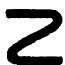
\includegraphics[keepaspectratio]{images/part001_a90573a3.jpg}}

命题 8. 设 \(f = \psi \circ g \circ \varphi\) 是连续映射 \(f: X \to Y\) 的典范分解，且设 \(R\) 表示等价关系

\[
f (x) = f (y).
\]

则下列三个条件等价：

\begin{enumerate}
\def\labelenumi{\alph{enumi})}
\item
  \(g\) 是由 \(\mathbf{X} / \mathbf{R}\) 到 \(f(\mathbf{X})\) 上的一个同胚。
\item
  在 \(f\) 之下，每个关于 \(\mathbf{R}\) 饱和的开集的像是子空间 \(f(\mathbf{X})\) 中的一个开集。
\item
  在 \(f\) 之下，每个关于 \(\mathbf{R}\) 饱和的闭集的像是子空间 \(f(\mathbf{X})\) 中的一个闭集。
\end{enumerate}

因为条件 b){[}resp. c){]}表达的是：X/R 中每个开（相应地，闭）集在 g 下的像是 \(f(\mathbf{X})\) 中的一个开（相应地，闭）集。

例。设 X 是拓扑空间，\((\mathbf{X}_{i})_{i\in I}\) 是 X 的一个覆盖，Y 是 X 的诸子空间 \(X_{v}\) 的和；则存在 Y 的一个分成既开又闭的子空间的分拆 \((\mathbf{Y}_{i})_{i\in I}\)，且对每个 \(i\in I\) 存在一个同胚 \(f_{i}:Y_{i}\to X_{i}\)。设 \(f:Y\to X\) 是与 \(f_{i}\)（在 \(Y_{i}\) 上，对每个 \(i\in I\)）相一致的连续映射，且设 R 是等价关系 \(f(x)=f(y)\)；于是商空间 Y/R 是把诸 \(Y_{i}\)"粘合"在一起得到的（§2，第 5 目）。考虑与 f 相伴的双射 \(g:Y/R\to X\)；一般说来 g 不是同胚，如下例所示：每个 \(X_{i}\) 都由单个点组成而 X 不是离散的。然而，若诸 \(X_{i}\) 的内部覆盖 X，或 \((\mathbf{X}_{i})\) 是 X 的一个局部有限闭覆盖，则 g 是同胚：因为若 U 是 Y 的任一关于 R 饱和的开子集，则对每个 \(i\in I\)，集合

\[
f (\mathbf {U}) \cap \mathbf {X} _ {i} = f _ {i} (\mathbf {U} \cap \mathbf {Y} _ {i})
\]

在 \(X_{i}\) 中是开集，且断言由第 1 目命题 3 得出。

下面的命题给出 \(g\) 是同胚的一个简单充分条件：

命题 9. 设 \(f: \mathbf{X} \to \mathbf{Y}\) 是一个连续满射，且设 \(\mathbf{R}\) 表示等价关系 \(f(x) = f(y)\)。若存在连续截面 \(s: \mathbf{Y} \to \mathbf{X}\)（与 \(f\) 相伴（《集合论》第二章，§ 3，第 8 目，定义 11）），则映射 \(g: \mathbf{X} / \mathbf{R} \to \mathbf{Y}\)（与 \(f\) 相伴）是一个同胚，且 \(s\) 是由 \(\mathbf{Y}\) 到子空间 \(s(\mathbf{Y})\)（\(\mathbf{X}\) 的子空间）上的一个同胚。

因为若 \(\varphi: \mathbf{X} \to \mathbf{X} / \mathbf{R}\) 是典范映射，则 \(g\) 与 \(\varphi \circ s\) 都是双射、连续且互逆；同样，\(s\) 与 \(f\) 在 \(s(\mathbf{Y})\) 上的限制都是双射、连续且互逆。

若 R 是拓扑空间 X 上的一个等价关系，且

\[
\varphi : \mathbf {X} \rightarrow \mathbf {X} / \mathbf {R}
\]

是典范映射，连续截面 \(s: \mathbf{X} / \mathbf{R} \to \mathbf{X}\)（与 \(\varphi\) 相伴）也称为 \(\mathbf{X}\) 关于 \(\mathbf{R}\) 的连续截面（参见《集合论》第二章，§ 6，第 2 目）；于是子空间 \(s(\mathbf{X} / \mathbf{R})\)（\(\mathbf{X}\) 的子空间）同胚于 \(\mathbf{X} / \mathbf{R}\)。若给定了 \(s(\mathbf{X} / \mathbf{R})\)，则 \(s\) 被唯一确定；\(s(\mathbf{X} / \mathbf{R})\) 常被（滥用语言地）称为 \(\mathbf{X}\) 关于 \(\mathbf{R}\) 的一个（连续）截面。

\pandocbounded{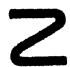
\includegraphics[keepaspectratio]{images/part001_feb98675.jpg}}

拓扑空间关于一个等价关系的连续截面未必存在（习题 12）。

\subsection{子空间的商空间}

设 X 是拓扑空间，A 是 X 的一个子空间，R 是 X 上的一个等价关系，f 是典范映射 \(X \to X/R\)，g 是 f 在 A 上的限制。A 上的等价关系 \(g(x) = g(y)\) 恰是 R 在 A 上诱导的关系 \(R_{A}\)（《集合论》R，§ 5，第 5 目）。设 \(g = \psi \circ h \circ \varphi\) 是 g 的典范分解，于是若 j 是 A 到 X 中的典范单射，我们就有一个交换图 (*)

\begin{enumerate}
\def\labelenumi{(\Roman{enumi})}
\tightlist
\item
\end{enumerate}

\pandocbounded{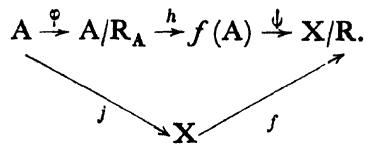
\includegraphics[keepaspectratio]{images/part001_6dc64900.jpg}}

命题 10. 典范双射 \(h: \mathbf{A} / \mathbf{R}_{\mathbf{A}} \to f(\mathbf{A})\) 是连续的。此外，下列三个命题等价：

\begin{enumerate}
\def\labelenumi{\alph{enumi})}
\item
  \(h\) 是一个同胚。
\item
  A 的每个关于 \(R_{A}\) 饱和的开子集都是 X 的某个关于 R 饱和的开子集与 A 的交。
\item
  A 的每个关于 \(R_{A}\) 饱和的闭子集都是 X 的某个关于 R 饱和的闭子集与 A 的交。
\end{enumerate}

命题的第一部分是直接的（第 5 目）。第二部分由第 5 目命题 8 得出：若 B 是 A 的关于 \(R_{A}\) 饱和的开（相应地，闭）子集，且 \(g(B) = f(B)\) 是 X/R 的某个开（相应地，闭）子集 C 与 \(f(A)\) 的交，则 B 是开（相应地，闭）子集 \(\overline{f}(C)\)

与 A 的交，该子集关于 R 饱和；反之，若 B 是某个关于 R 饱和的开（相应地，闭）子集 D 与 A 的交，则 \(f(\mathbf{B})\) 是 \(f(\mathbf{A})\) 与 \(f(\mathbf{D})\) 的交，而它在 X/R 中是开（相应地，闭）集。

推论 1. 若 A 是 X 的关于 R 饱和的开（相应地，闭）子集，则典范映射 \(h: \mathrm{A}/\mathrm{R}_{\mathrm{A}} \rightarrow f(\mathrm{A})\) 是一个同胚。

因为若 A 在 X 中开（相应地，闭）且关于 R 饱和，且 \(B \subset A\) 在 A 中开（相应地，闭）且关于 \(R_{A}\) 饱和，则 B 在 X 中开（相应地，闭）且关于 R 饱和。

推论 2. 若存在连续映射 \(u: \mathbf{X} \to \mathbf{A}\)，使得 \(u(x)\) 与 \(x \mod \mathbb{R}\) 同余（对每个 \(x \in \mathbf{X}\)），则 \(f(\mathbf{A}) = \mathbf{X} / \mathbb{R}\)，且典范映射 \(h: \mathbf{A} / \mathbb{R}_{\mathbf{A}} \to \mathbf{X} / \mathbb{R}\) 是一个同胚。

由于模 R 的每个等价类都与 A 相交，\(A/R_{A}\) 在 X/R 中的典范像是整个 X/R；另一方面，若 U 在 A 中开且关于 \(R_{A}\) 饱和，则由假设可知，\(\overline{u}^{1}(U)\) 是把 U 关于 R 饱和化所得到的集合；由于 u 连续，\(\overline{u}^{1}(U)\) 在 X 中是开集（§ 2，第 1 目，定理 1）。由这一事实并借助命题 10 即得推论。

例。* 设 R 表示实直线 R 上的等价关系 \(x \equiv y \pmod{1}\)（第 4 目，例），且设 A 表示闭区间 {[}0, 1{]}；A 包含模 R 每个等价类的至少一个点。\(\mathrm{A} / \mathbb{R}_{\mathbf{A}}\) 到环面 T 上的典范映射是一个同胚；因为若 F 在 A 中闭（从而在 R 中闭），则为把 F 关于关系 R 饱和化，须取诸闭集 \(\mathrm{F} + n\)（对所有 \(n \in \mathbf{Z}\)）的并，它们显然构成一个局部有限族，故其并是闭集（§ 1，第 5 目，命题 4）；断言由此得出。我们指出，\(\mathrm{A} / \mathbb{R}_{\mathbf{A}}\) 是把 A 中的点 0 与 1 等同起来得到的。*

\section{拓扑空间的积}

\subsection{积空间}

定义 1. 给定拓扑空间的一个族 \((\mathbf{X}_{t})_{t\in I}\)，这个族的积空间是指积集合 \(\mathbf{X} = \prod_{t\in I}\mathbf{X}_{t}\) 赋以诸 \(\mathbf{X}_{t}\) 的拓扑的积（§ 2，第 3 目，例 3）。诸空间 \(\mathbf{X}_{t}(t\in I)\) 称为 \(\mathbf{X}\) 的因子。

由 § 2 第 3 目命题 4，X 上的积拓扑以形如 \(\overline{\mathrm{pr}}_{t}^{1}(\mathbf{U}_{t})\) 的集合的有限交组成的集合 B 为一个基，其中 \(U_{t}\) 在 \(X_{t}\) 中是开集；这些集合是积 \(\prod_{i\in I}A_{i}\)，其中 \(A_{i}\) 在 \(X_{t}\) 中是开集（对每个 \(i\in I\)），且除去有限多个指标外 \(A_{i}=X_{t}\)。这些集合将称为初等集。

若 \(\mathfrak{B}_i\) 是 \(X_i\) 的拓扑的一个基（对每个 \(i \in I\)），则显然，初等集 \(\prod_{i \in I} A_i\)（满足 \(A_i \in \mathfrak{B}_i\)（对每个指标 \(i\)，只要 \(A_i \neq X_i\)））组成积拓扑的另一个基。于是，包含给定点 \(x \in X\) 的这种类型的初等集组成 \(x\) 的一个基本邻域系（\(\S 1\)，第 3 目，命题 3）。

若 I 是有限集，由诸因子 \(X_{i}\) 的拓扑构造积拓扑就更简单：初等集恰是积 \(\prod_{i\in I}A_{i}\)，其中 \(A_{i}\) 是 \(X_{i}\) 的任意开子集（对每个 \(i\in I\)）（参见习题 9）。

例。* 积 \(\mathbf{R}^n\)（\(n\) 个与实直线 \(\mathbf{R}\) 恒同的空间的积）称为 \(n\) 维实数空间；\(\mathbf{R}^2\) 也称为实平面（参见第六章，§ 1）。类似地，从有理直线 \(\mathbf{Q}\) 出发，我们定义 \(n\) 维有理数空间 \(\mathbf{Q}^n\)（当 \(n = 2\) 时称为有理平面）。

空间 \(\mathbf{R}^n\) 的拓扑以 \(n\) 个 \(\mathbf{R}\) 中开区间的所有积组成的集合为一个基，这些积称为 \(n\) 维开方块。包含点 \(x \in \mathbf{R}^n\) 的开方块组成这一点的一个基本邻域系。类似地，\(n\) 个 \(\mathbf{R}\) 中闭区间的积称为 \(n\) 维闭方块。以 \(x\) 为内点的闭方块也组成 \(x\) 的一个基本邻域系。对 \(\mathbf{Q}^n\) 有类似的结果。*

命题 1. 设 \(f = (f_{i})\) 是拓扑空间 \(Y\) 到积空间 \(X = \prod_{i \in I} X_{i}\) 中的一个映射。则 \(f\) 在点 \(a \in Y\) 处连续，当且仅当 \(f_{i}\)（对每个 \(i \in I\)）在 a 处连续。

由于 \(f_{t} = \mathrm{pr}_{t} \circ f\)，这只是 §2 第 3 目命题 4 的一个特例。

推论 1. 设 \((\mathbf{X}_t)_{i \in \mathbf{I}}\)、\((\mathbf{Y}_t)_{i \in \mathbf{I}}\) 是具有同一指标集的两个拓扑空间族。对每个 \(i \in \mathbf{I}\)，设 \(f_i\) 是 \(\mathbf{X}_t\) 到 \(\mathbf{Y}_t\) 中的一个映射。为使积映射 \(f: (x_i) \to (f_i(x_i))\)（它把

\[
\prod_ {i \in I} X _ {i} \quad i n t o \quad \prod_ {i \in I} Y _ {i}
\]

映到）在一点 \(a = (a_{i})\) 处连续，必须且只需 \(f_{i}\) 在 \(a_{i}\) 处连续（对每个 \(\mathfrak{t} \in \mathbf{I}\)）。

\(f\) 可以写成 \(x \to (f_{t}(\mathrm{pr}_{t}(x))\)，于是由命题 1，该条件是充分的。反之，对每个 \(x \in I\)，设 \(g_{x}\) 是 \(X_{x}\) 到 \(\prod_{i \in I} X_{i}\) 中的这样的映射：\(\mathrm{pr}_{x}(g_{x}(x_{x})) = x_{x}\)，且 \(\mathrm{pr}_{t}(g_{x}(x_{x})) = a_{t}\)（每当 \(i \neq x\)）；则由命题 1，\(g_{x}\) 在点 \(a_{x}\) 处连续。由于 \(f_{x} = \mathrm{pr}_{x} \circ f \circ g_{x}\)，由此得出：若 \(f\) 在 \(a\) 处连续，则 \(f_{x}\) 在 \(a_{x}\) 处连续。

推论 2. 设 X、Y 是两个拓扑空间。为使映射 \(f: \mathbf{X} \to \mathbf{Y}\) 连续，必须且只需映射 \(g: x \to (x, f(x))\) 是 X 到 \(f\) 的图象 G 上（把 G 看作积空间 \(\mathbf{X} \times \mathbf{Y}\) 的子空间）的一个同胚。

由于 \(f = \mathrm{pr}_2 \circ g\)，该条件是充分的。它也是必要的，因为若 \(f\) 连续，则 \(g\) 是双射且连续（命题 1），且 \(g\) 的逆是 \(\mathrm{pr}_1\) 在 \(G\) 上的限制，它是连续的（参见《集合论》第四章，§ 2，第 4 目，判别准则 CST 17）。

命题 2（拓扑积的结合性）. 设 \((\mathbf{X}_{\iota})_{\iota \in \mathbf{I}}\) 是拓扑空间的一个族，\((\mathbf{J}_{\kappa})_{\kappa \in \mathbf{K}}\) 是集合 I 的一个分拆，且对每个 \(\kappa \in \mathbf{K}\)，设 \(\mathbf{X}_{\kappa}^{\prime} = \prod_{i\in \mathbf{J}_{\kappa}}\mathbf{X}_{\iota}\) 是诸空间 \(\mathbf{X}_{\iota}\)（对 \(\iota \in \mathbf{J}_{\mathbf{K}}\)）的积。则积空间的典范映射
